\chapter{Resultados para una sigmoide}\label{anx:1}
\subsection*{Variando el parámetro $r_{i,min}$}

\begin{figure}[htbp]
  \centering
  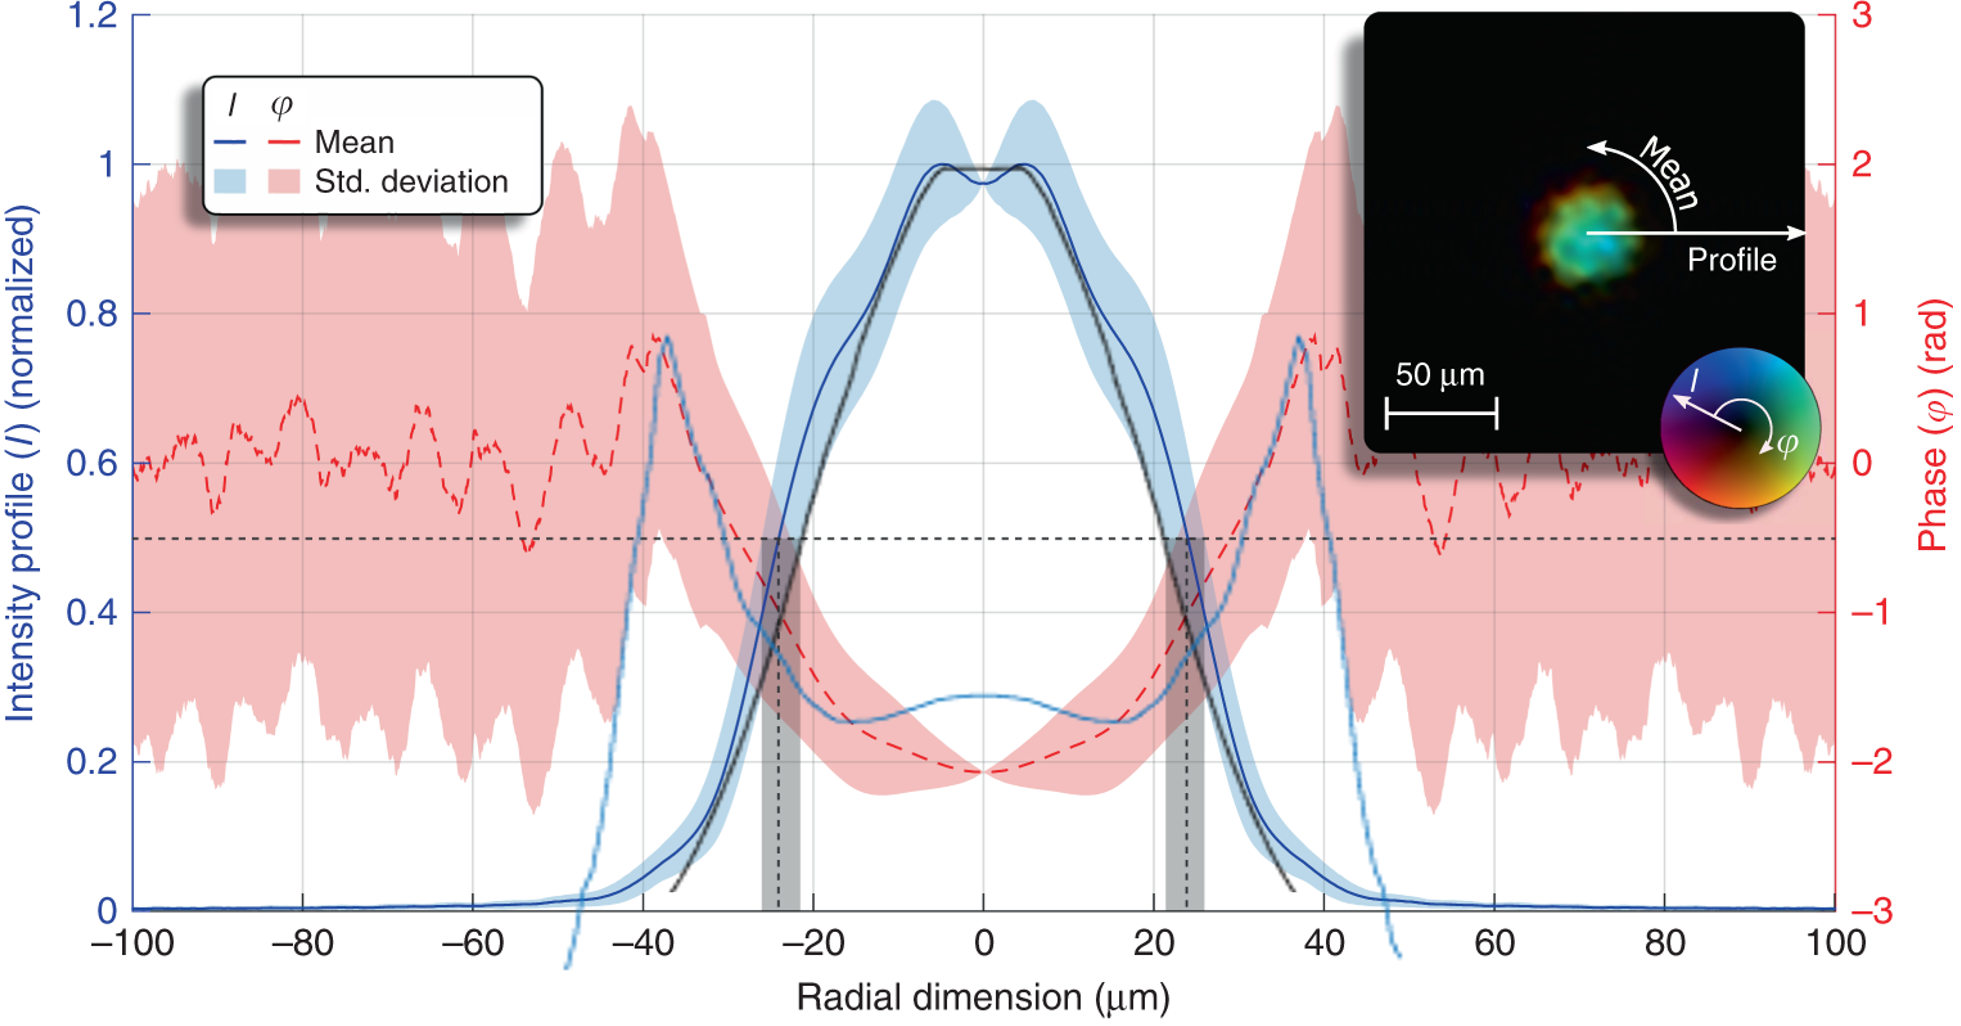
\includegraphics[width=0.75\textwidth]{Figuras/anx_cmp_11.png}
  \caption*{Comparación entre los perfiles radiales de intensidad--fase con $r_{i,min}=\qty{0}{µm}$ y $r_{i,max}=\qty{5}{µm}$, manteniendo los valores de los parámetros $k_{i}=\qty{50e6}{m^{-1}}$ y $z_{0i}=\qty{3.8}{mm}$; y el experimento.}
\end{figure}

\begin{figure}[htbp]
  \centering
  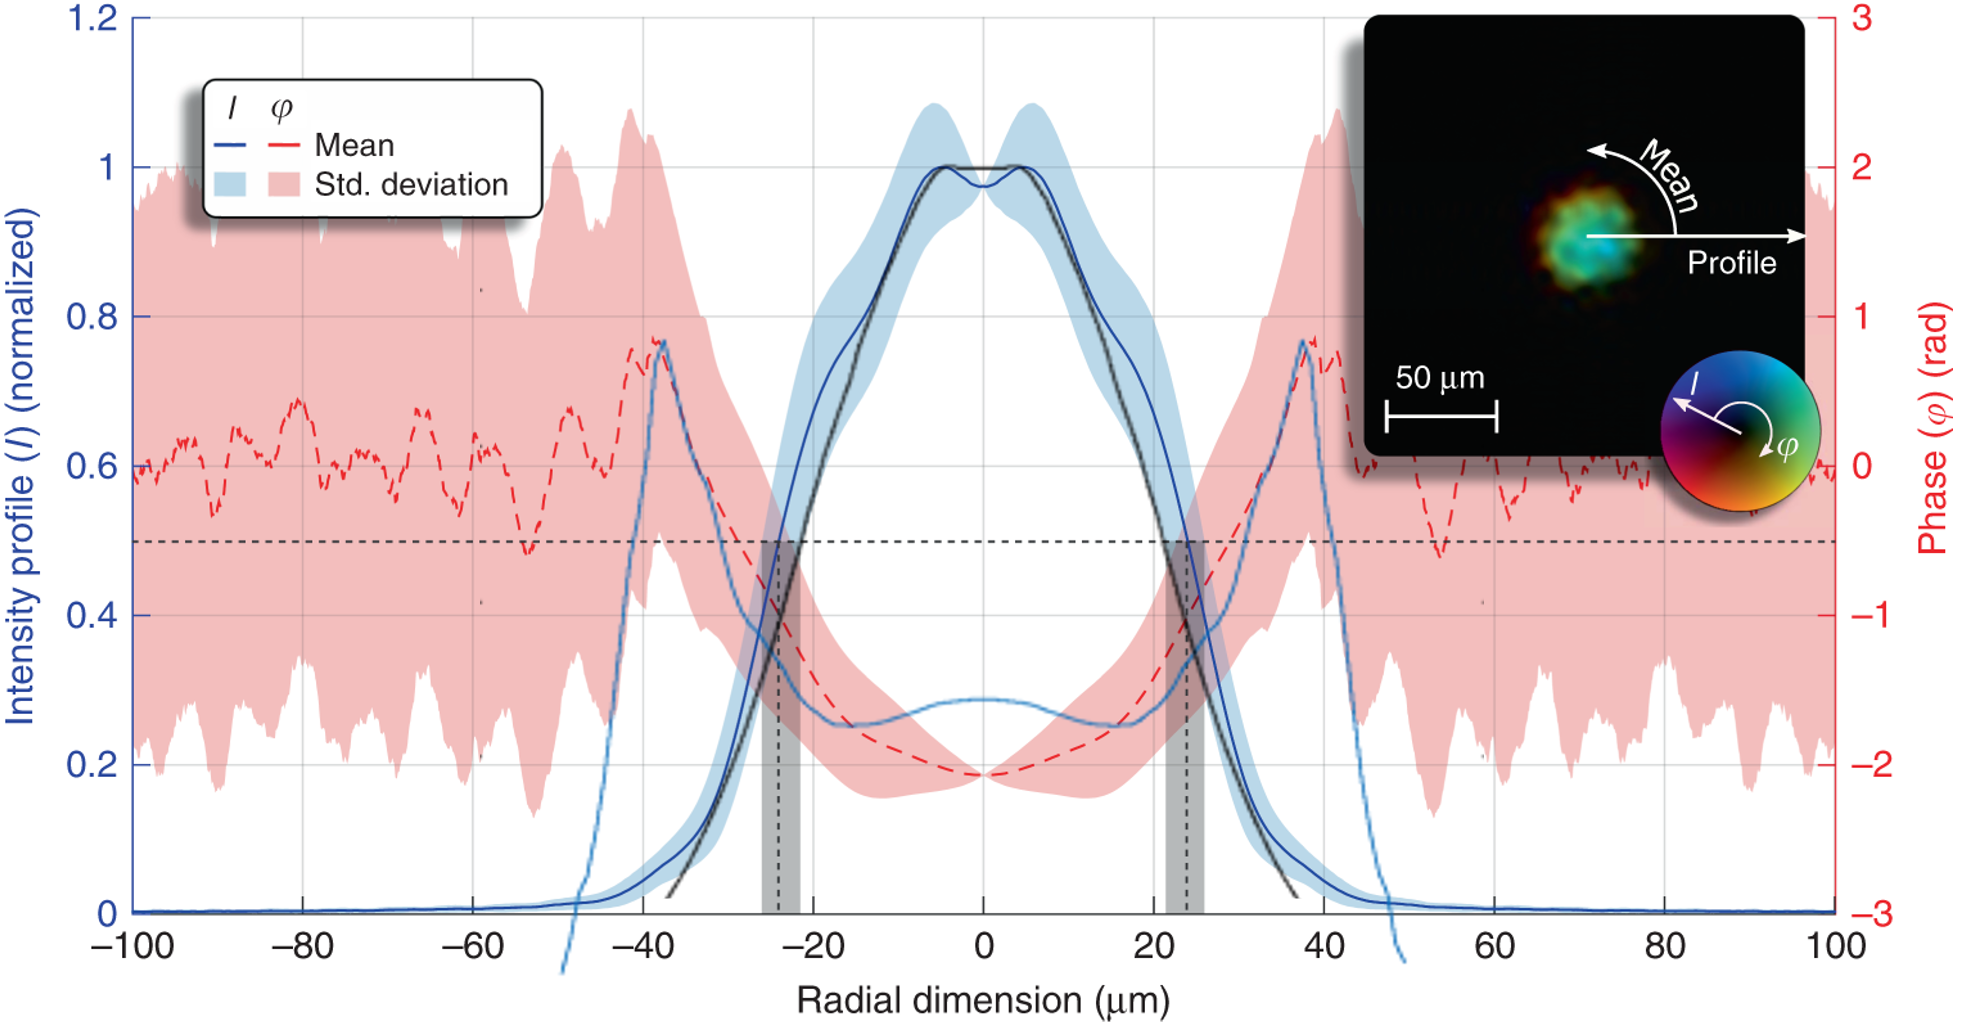
\includegraphics[width=0.75\textwidth]{Figuras/anx_cmp_12.png}
  \caption*{Comparación entre los perfiles radiales de intensidad--fase con $r_{i,min}=\qty{1}{µm}$ y $r_{i,max}=\qty{5}{µm}$, manteniendo los valores de los parámetros $k_{i}=\qty{50e6}{m^{-1}}$ y $z_{0i}=\qty{3.8}{mm}$; y el experimento.}
\end{figure}

\newpage

\begin{figure}[htbp]
  \centering
  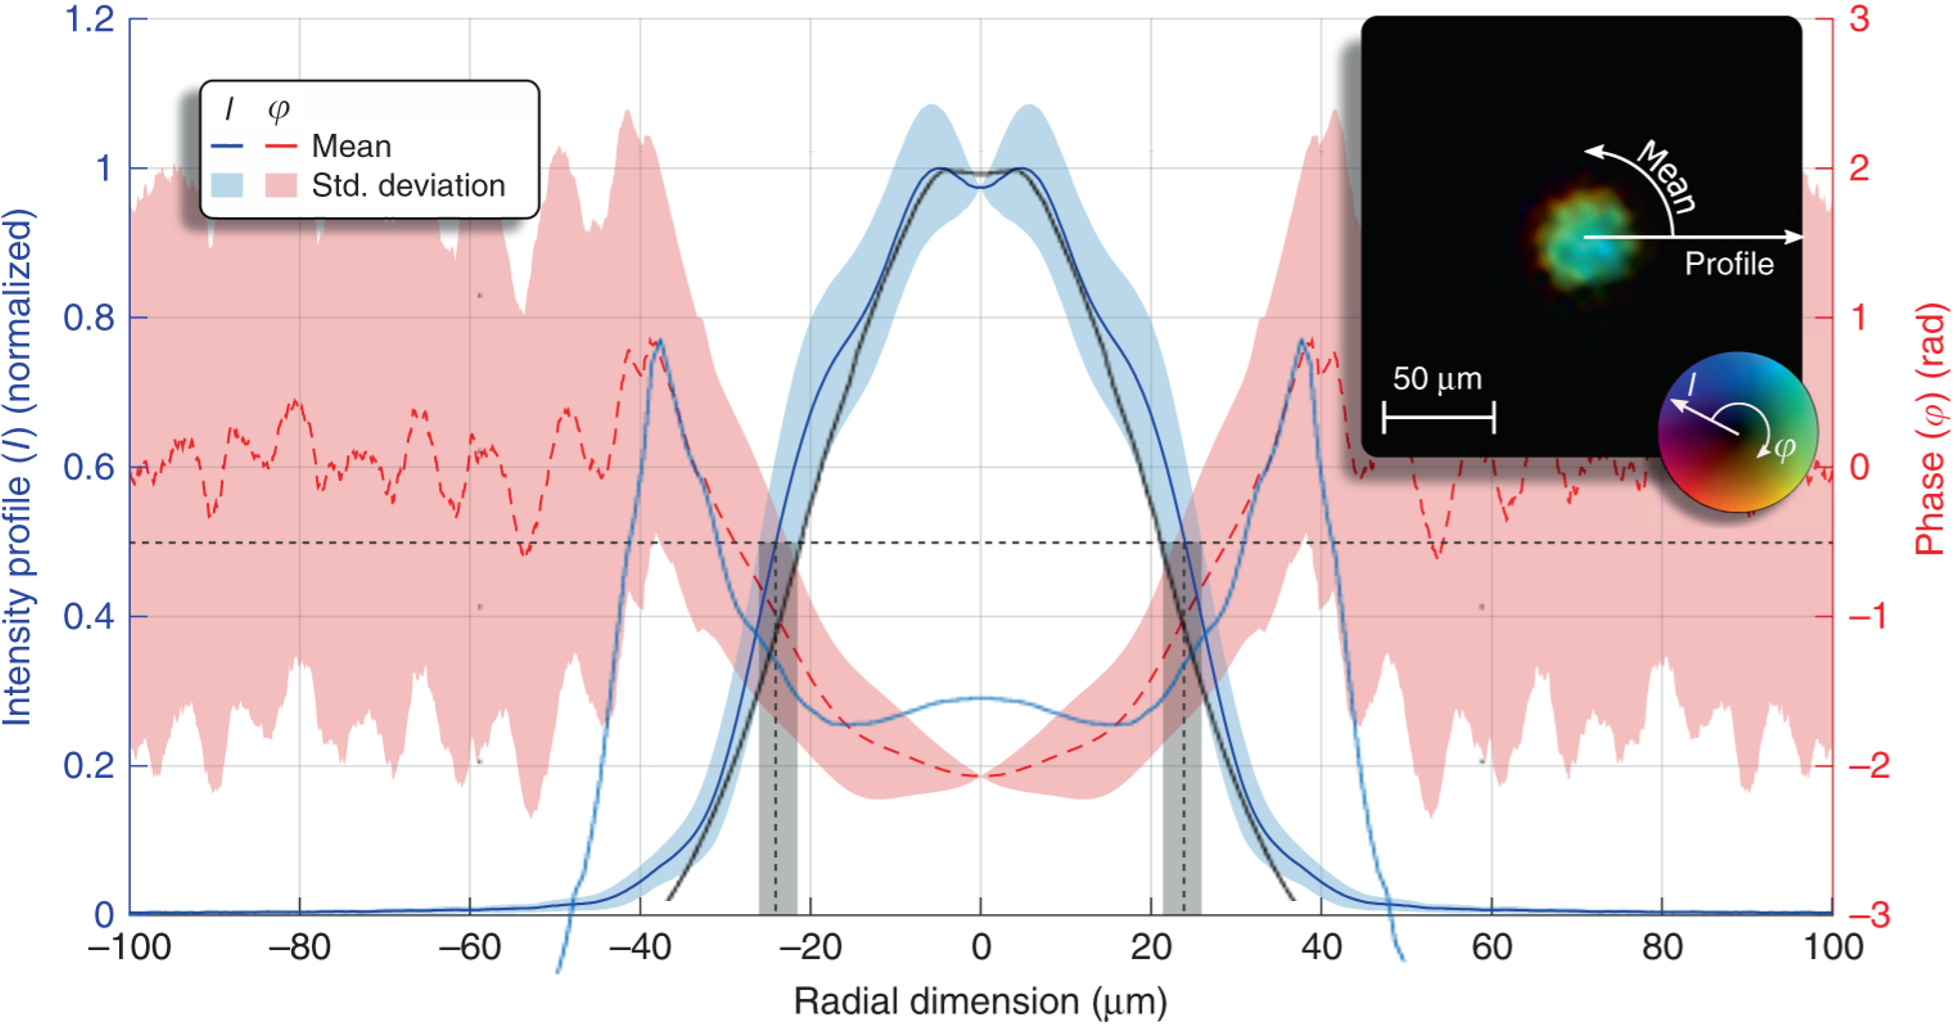
\includegraphics[width=0.74\textwidth]{Figuras/anx_cmp_13.png}
  \caption*{Comparación entre los perfiles radiales de intensidad--fase con $r_{i,min}=\qty{2}{µm}$ y $r_{i,max}=\qty{5}{µm}$, manteniendo los valores de los parámetros $k_{i}=\qty{50e6}{m^{-1}}$ y $z_{0i}=\qty{3.8}{mm}$; y el experimento.}
\end{figure}

\begin{figure}[htbp]
  \centering
  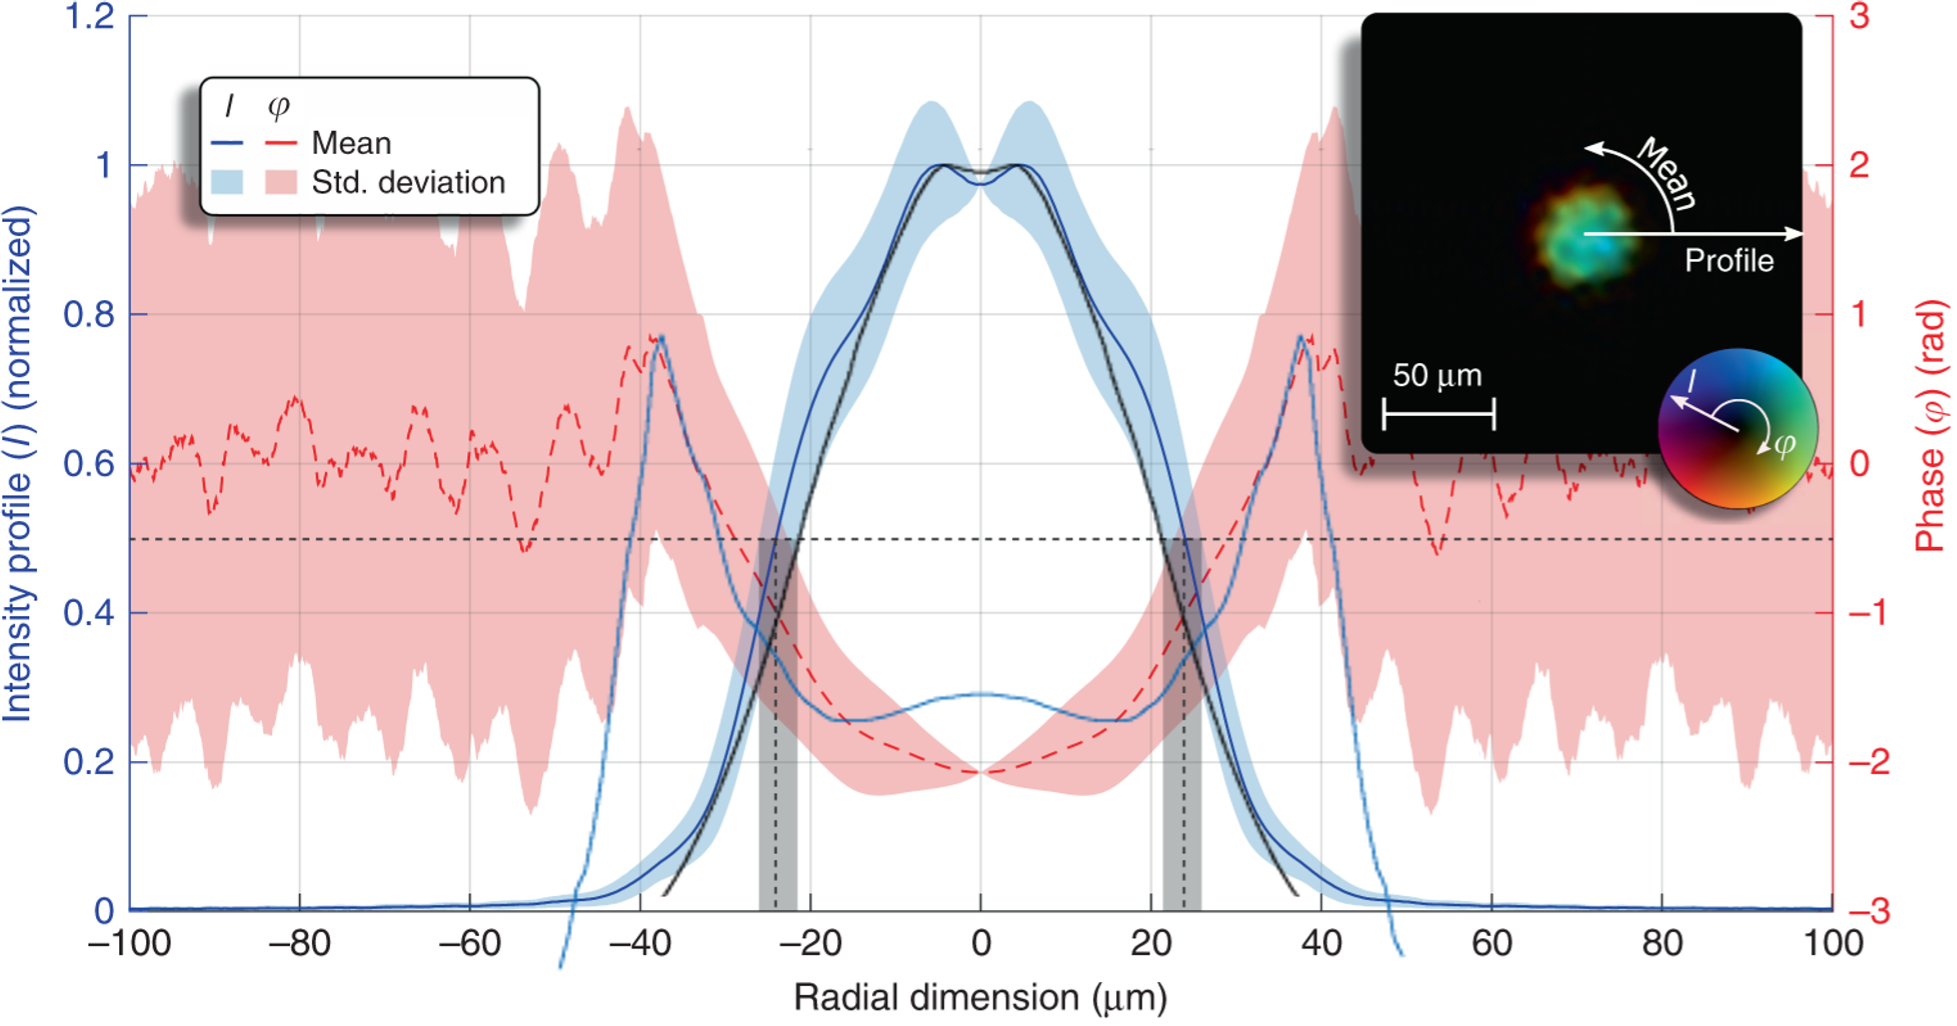
\includegraphics[width=0.74\textwidth]{Figuras/anx_cmp_14.png}
  \caption*{Comparación entre los perfiles radiales de intensidad--fase con $r_{i,min}=\qty{3}{µm}$ y $r_{i,max}=\qty{5}{µm}$, manteniendo los valores de los parámetros $k_{i}=\qty{50e6}{m^{-1}}$ y $z_{0i}=\qty{3.8}{mm}$; y el experimento.}
\end{figure}

\begin{figure}[htbp!]
  \centering
  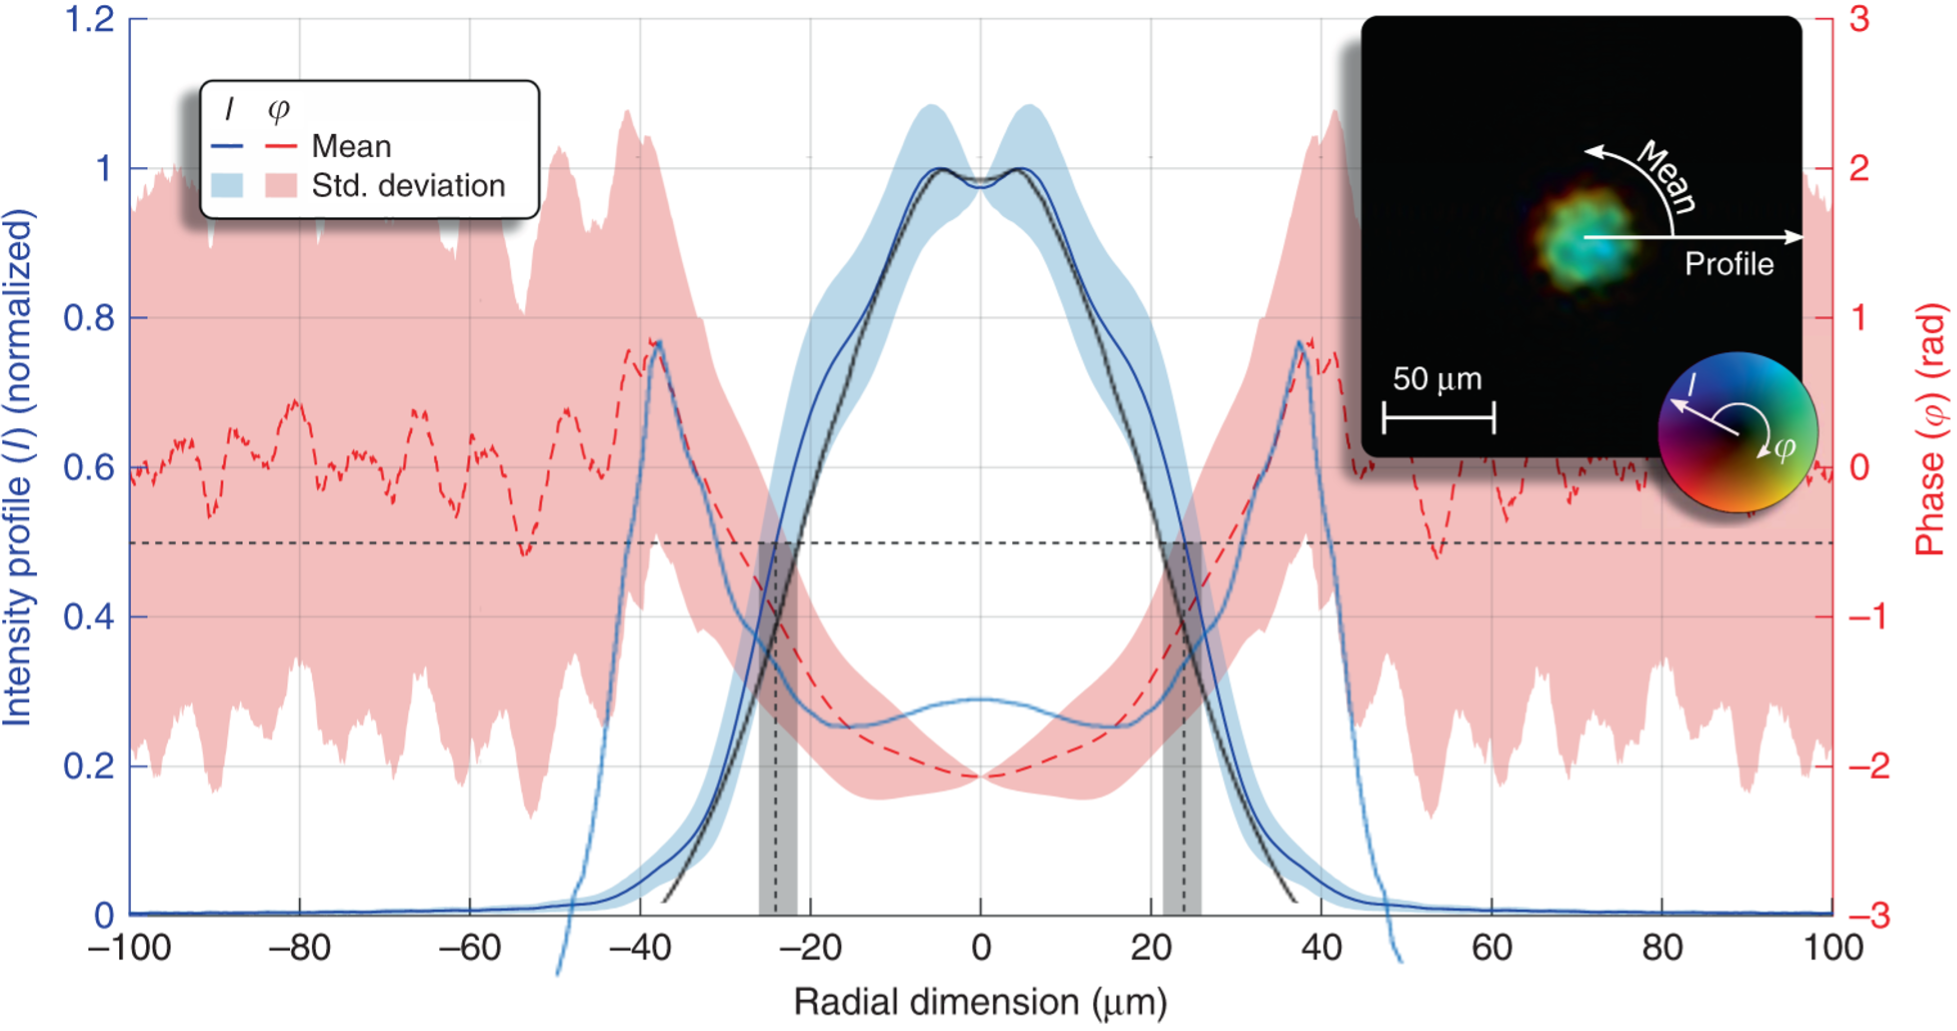
\includegraphics[width=0.74\textwidth]{Figuras/anx_cmp_15.png}
  \caption*{Comparación entre los perfiles radiales de intensidad--fase con $r_{i,min}=\qty{4}{µm}$ y $r_{i,max}=\qty{5}{µm}$, manteniendo los valores de los parámetros $k_{i}=\qty{50e6}{m^{-1}}$ y $z_{0i}=\qty{3.8}{mm}$; y el experimento.}
\end{figure}

\newpage

\begin{figure}[htbp]
  \centering
  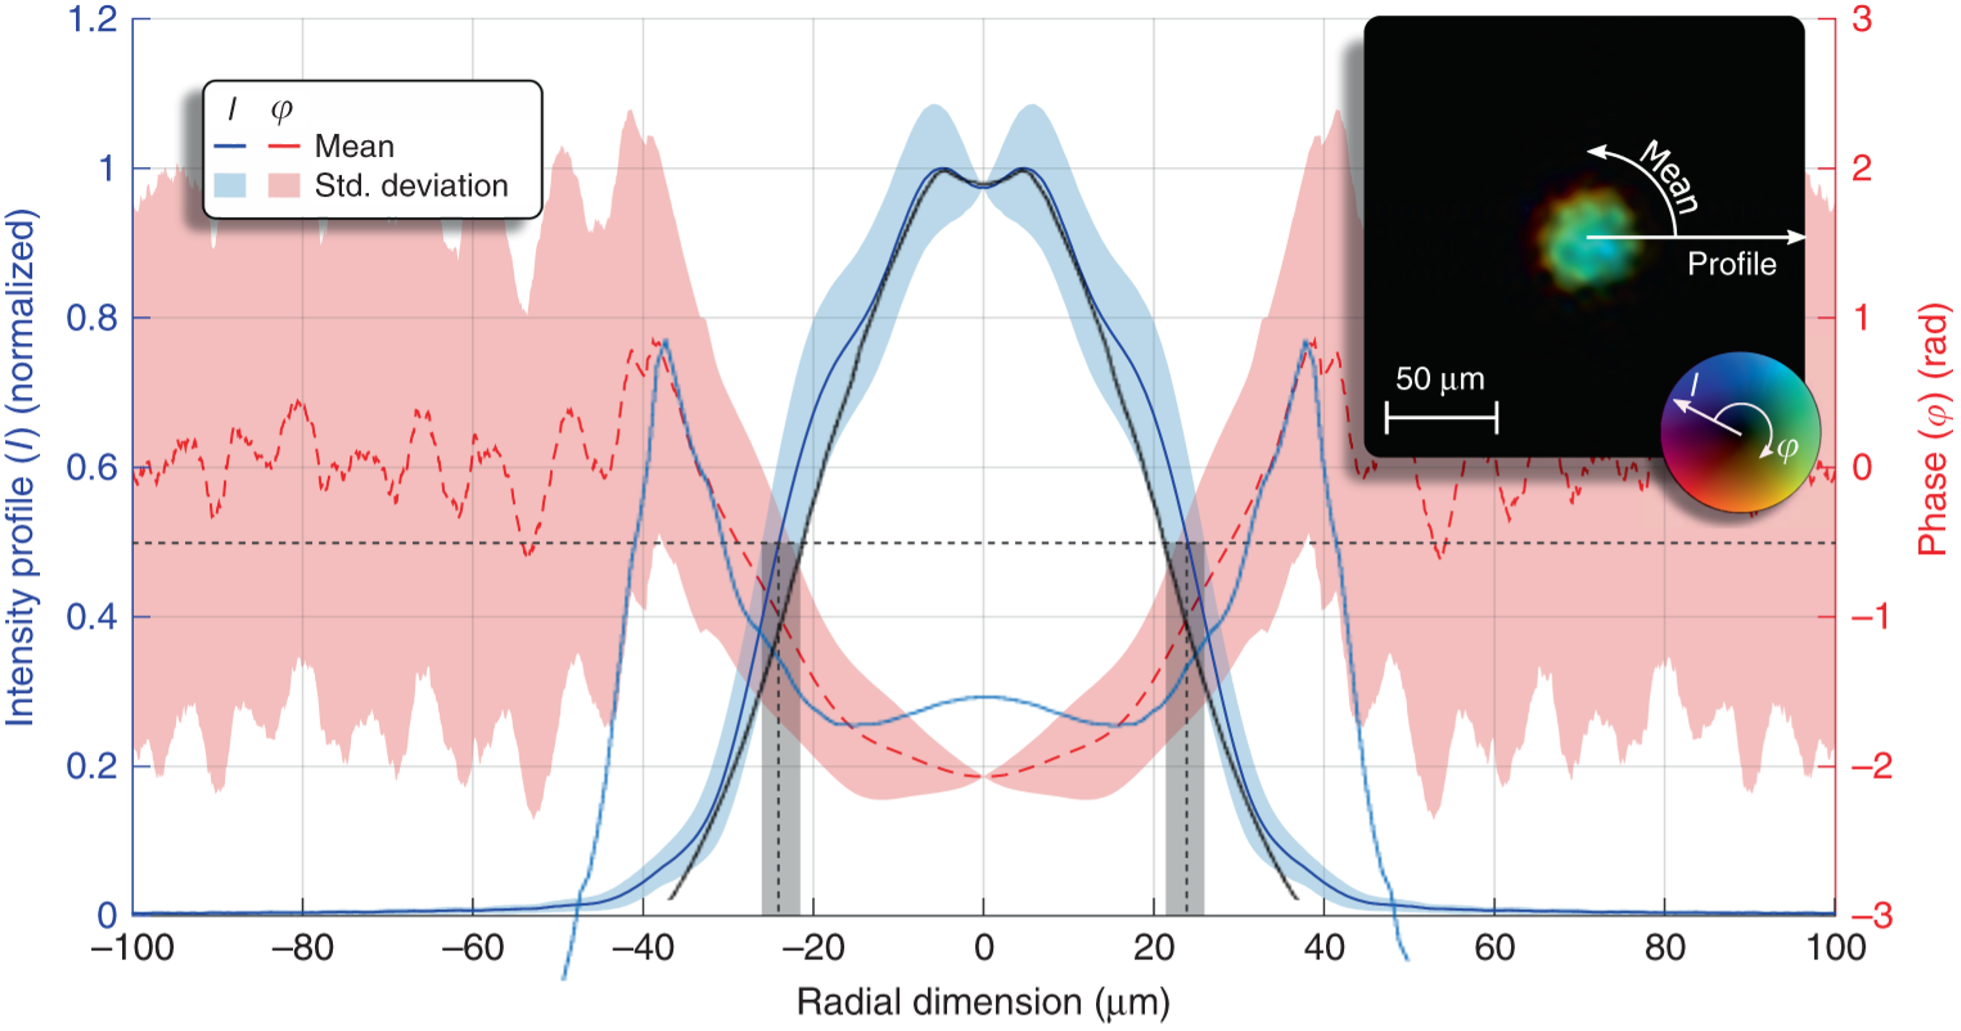
\includegraphics[width=0.75\textwidth]{Figuras/anx_cmp_16.png}
  \caption*{Comparación entre los perfiles radiales de intensidad--fase con $r_{i,min}=\qty{5}{µm}$ y $r_{i,max}=\qty{5}{µm}$, manteniendo los valores de los parámetros $k_{i}=\qty{50e6}{m^{-1}}$ y $z_{0i}=\qty{3.8}{mm}$; y el experimento.}
\end{figure}

\subsection*{Variando el parámetro $z_{0i}$}

\begin{figure}[htbp]
  \centering
  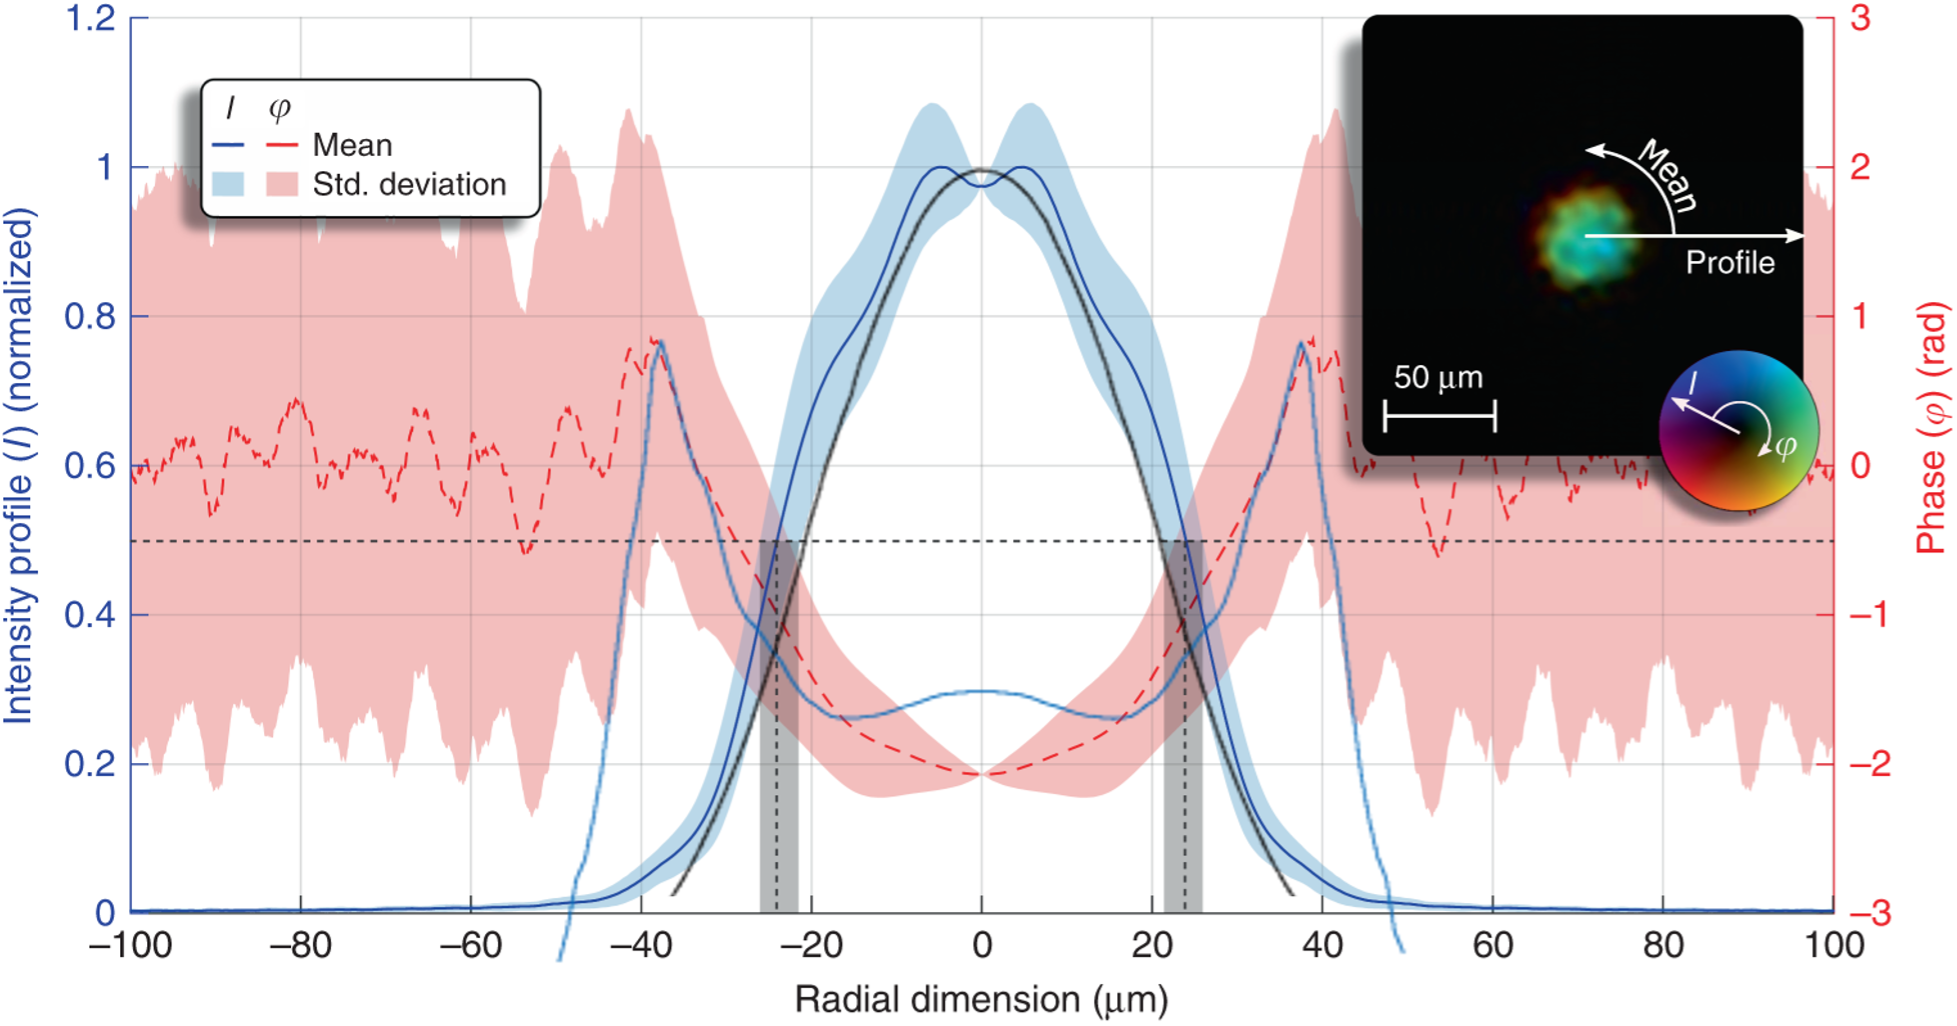
\includegraphics[width=0.7\textwidth]{Figuras/anx_cmp_21.png}
  \caption*{Comparación entre los perfiles radiales de intensidad--fase con $z_{0i}=\qty{2}{mm}$, manteniendo los valores de los parámetros $r_{i,min}=\qty{0}{µm}$, $r_{i,max}=\qty{5}{µm}$ y $k_{i}=\qty{50e6}{m^{-1}}$; y el experimento.}
\end{figure}

\begin{figure}[htbp!]
  \centering
  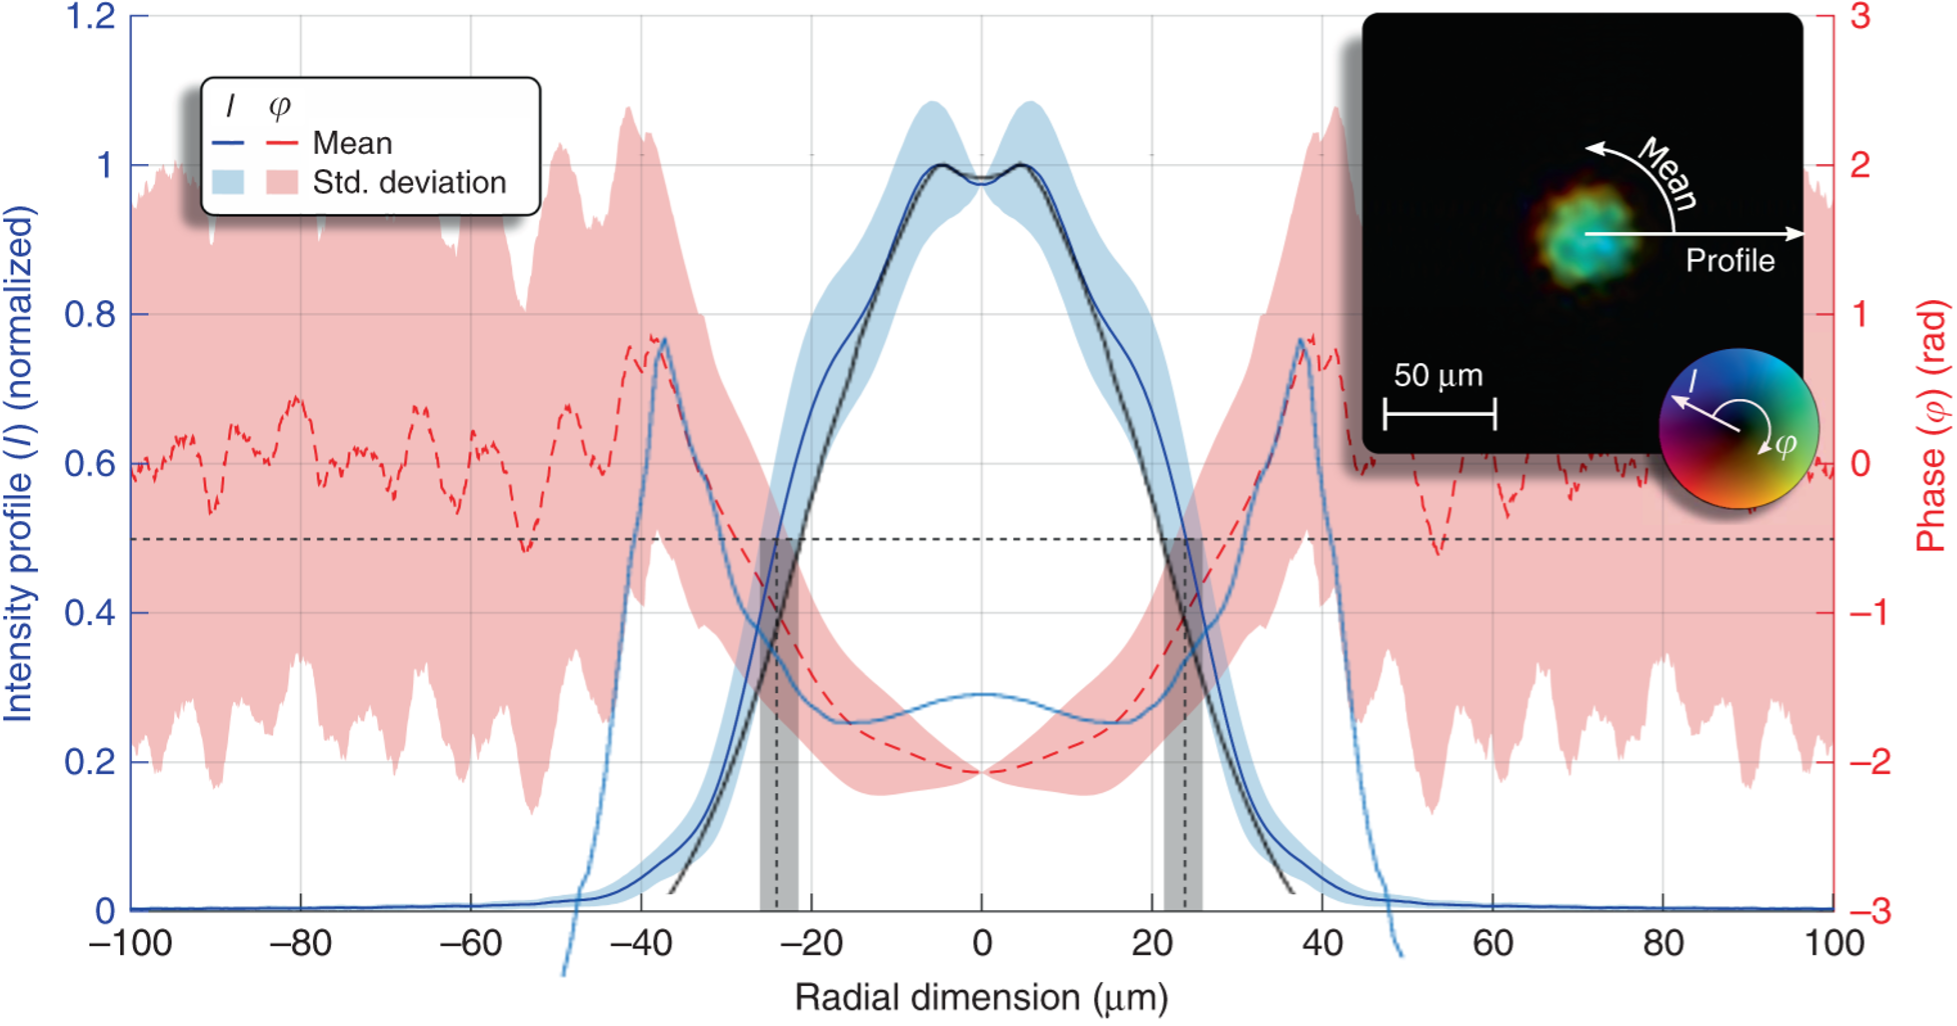
\includegraphics[width=0.7\textwidth]{Figuras/anx_cmp_22.png}
  \caption*{Comparación entre los perfiles radiales de intensidad--fase con $z_{0i}=\qty{2}{mm}$, manteniendo los valores de los parámetros $r_{i,min}=\qty{5}{µm}$, $r_{i,max}=\qty{5}{µm}$ y $k_{i}=\qty{50e6}{m^{-1}}$; y el experimento.}
\end{figure}

\begin{figure}[htbp]
  \centering
  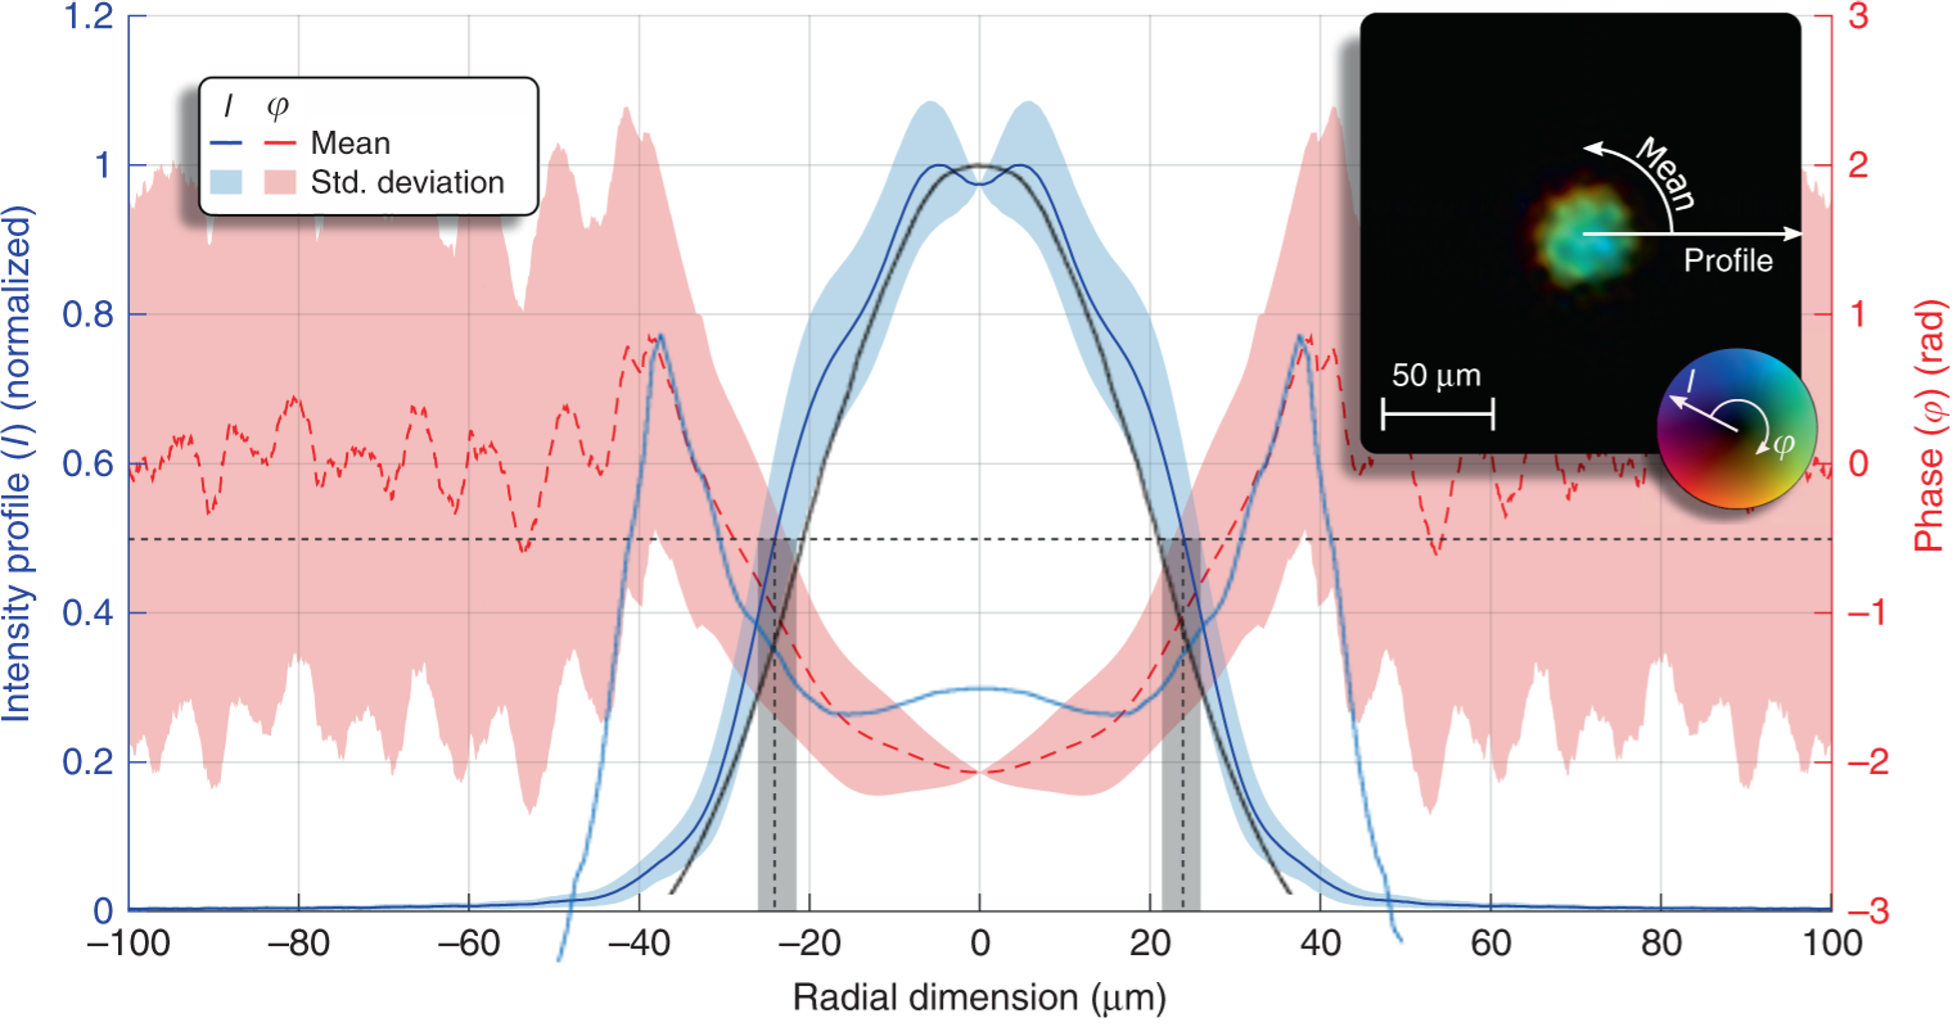
\includegraphics[width=0.74\textwidth]{Figuras/anx_cmp_23.png}
  \caption*{Comparación entre los perfiles radiales de intensidad--fase con $z_{0i}=\qty{2.5}{mm}$, manteniendo los valores de los parámetros $r_{i,min}=\qty{0}{µm}$, $r_{i,max}=\qty{5}{µm}$ y $k_{i}=\qty{50e6}{m^{-1}}$; y el experimento.}
\end{figure}

\begin{figure}[htbp]
  \centering
  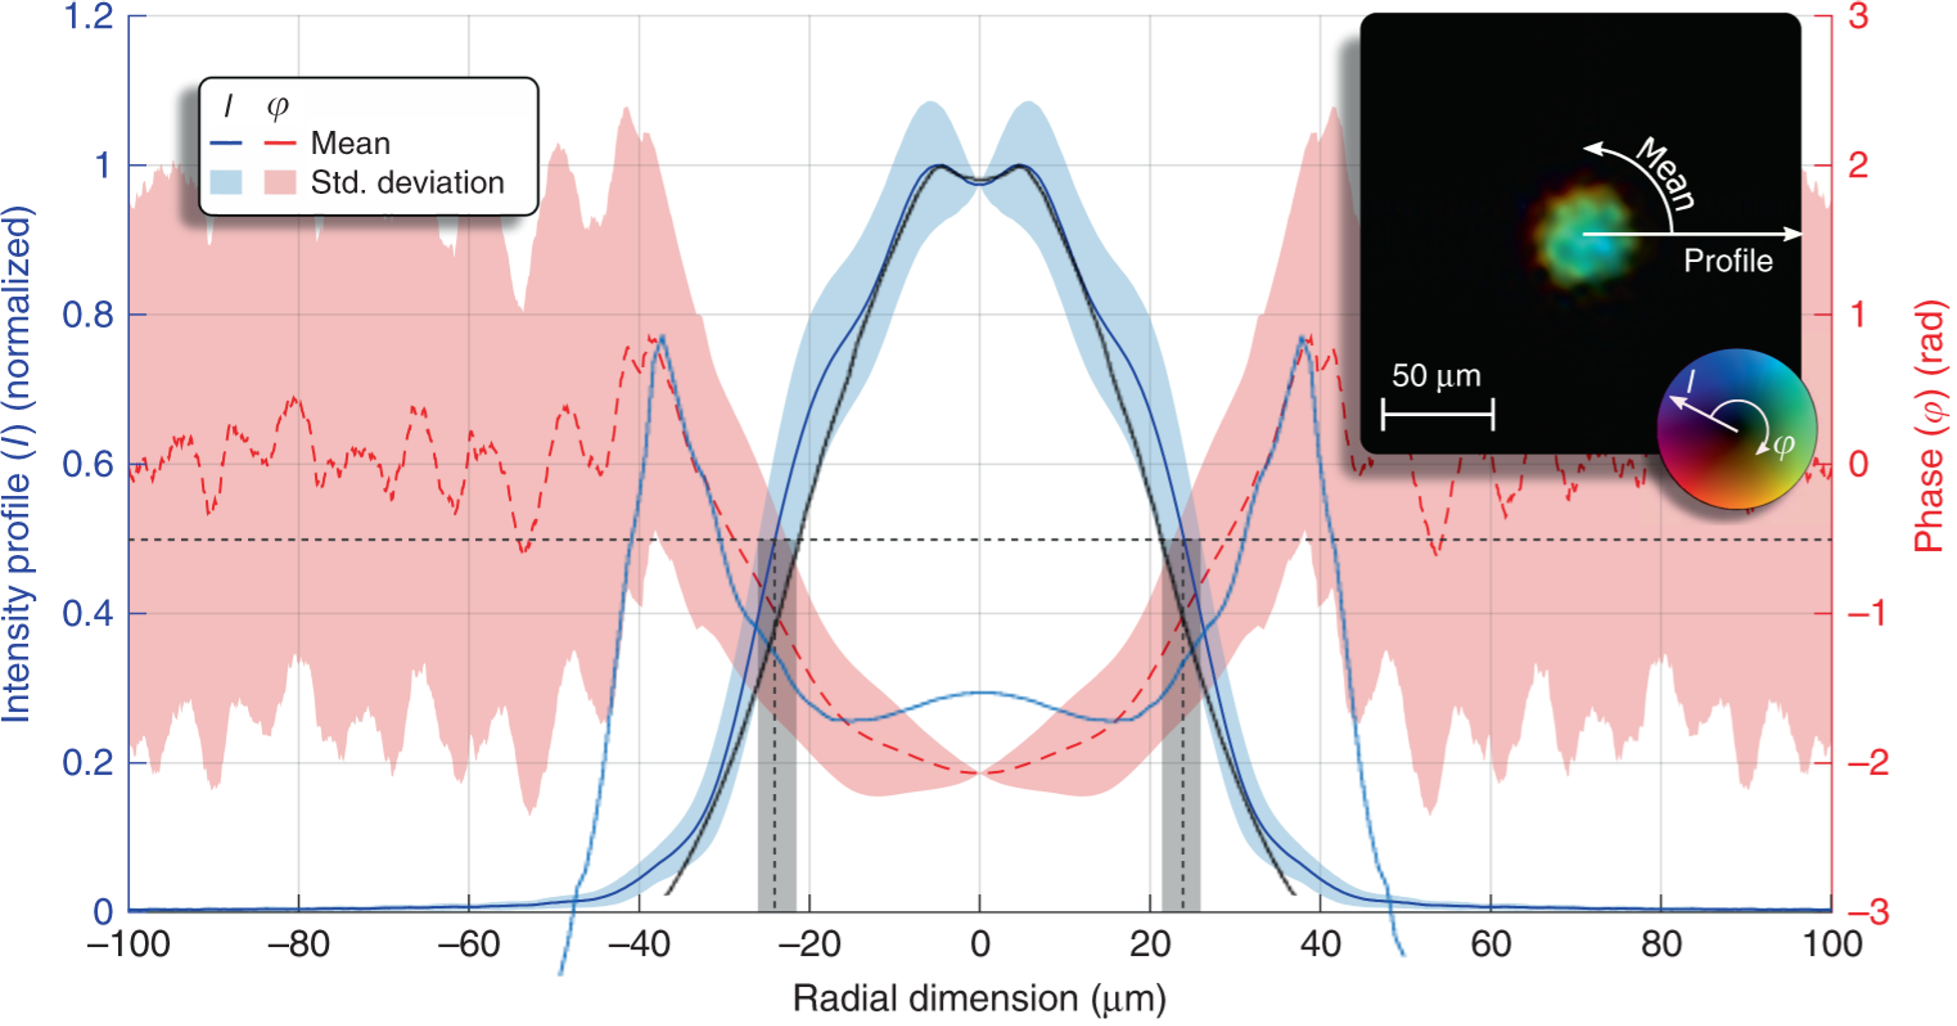
\includegraphics[width=0.74\textwidth]{Figuras/anx_cmp_24.png}
  \caption*{Comparación entre los perfiles radiales de intensidad--fase con $z_{0i}=\qty{2.5}{mm}$, manteniendo los valores de los parámetros $r_{i,min}=\qty{5}{µm}$, $r_{i,max}=\qty{5}{µm}$ y $k_{i}=\qty{50e6}{m^{-1}}$; y el experimento.}
\end{figure}

\begin{figure}[htbp]
  \centering
  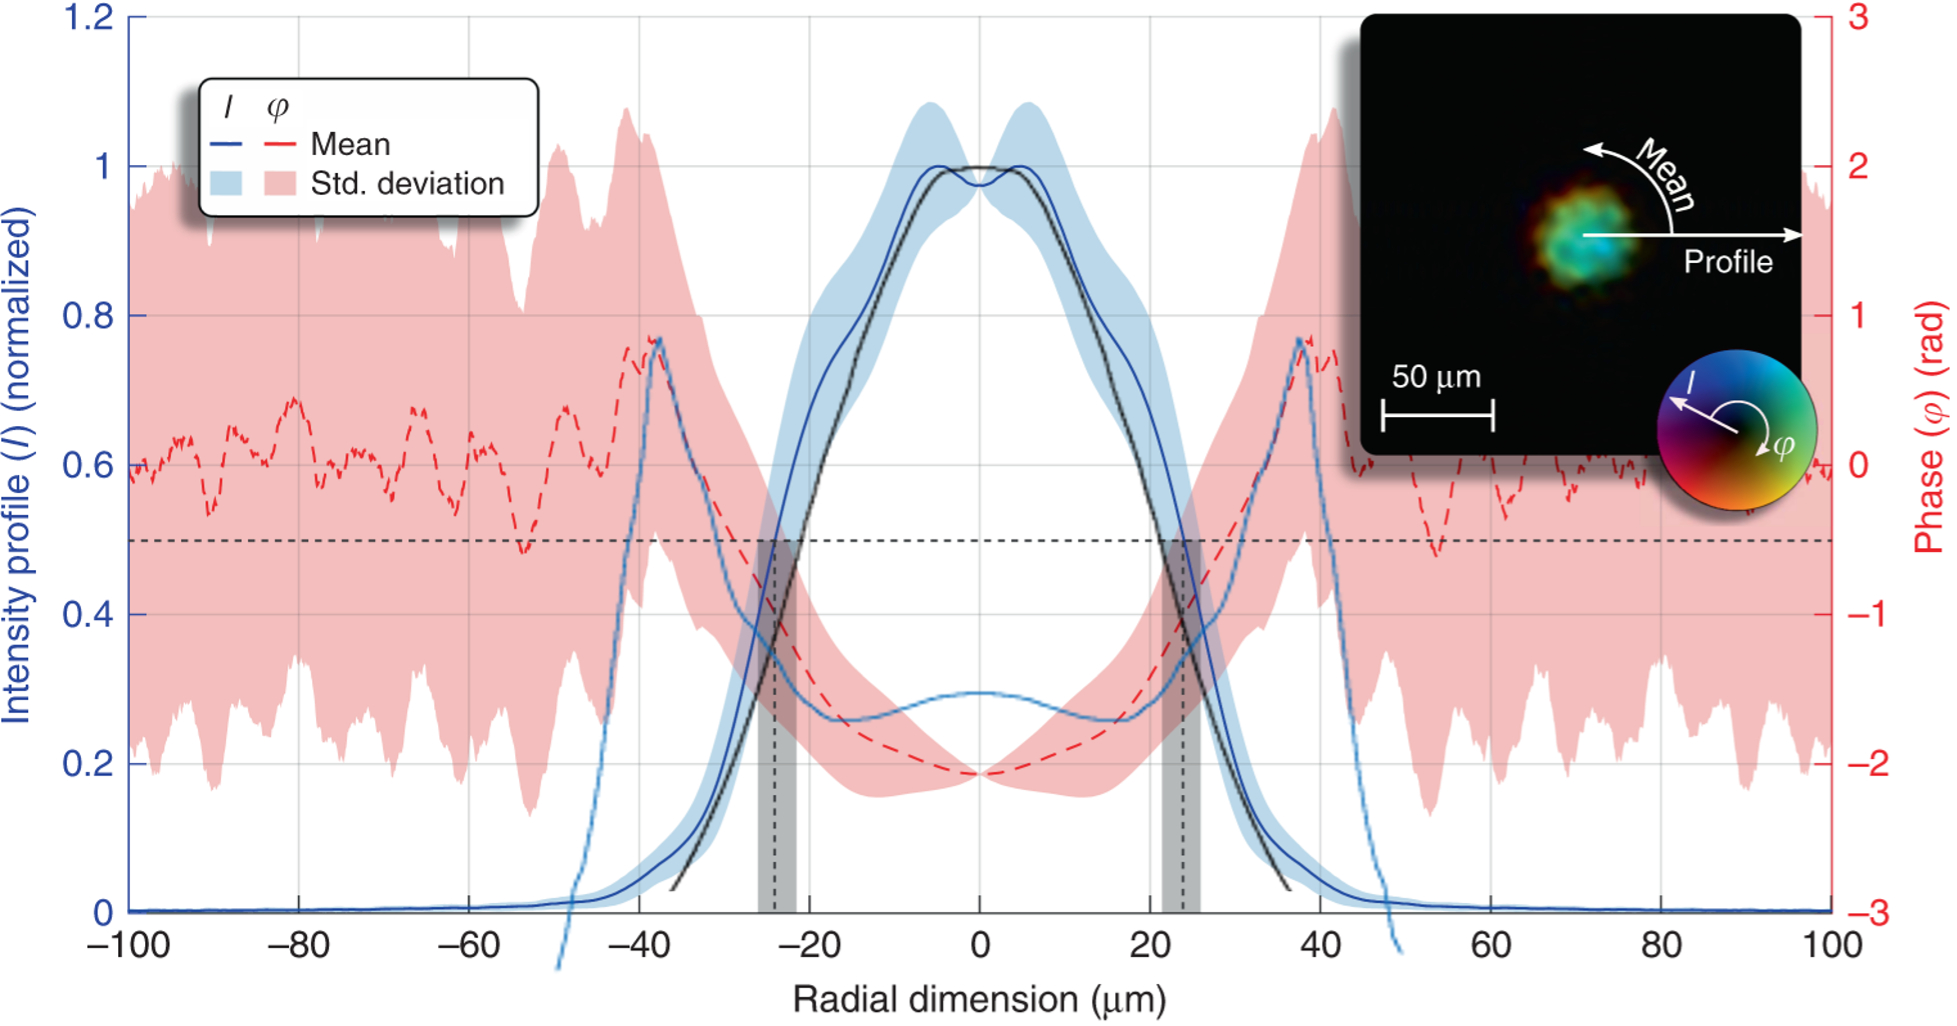
\includegraphics[width=0.74\textwidth]{Figuras/anx_cmp_25.png}
  \caption*{Comparación entre los perfiles radiales de intensidad--fase con $z_{0i}=\qty{3}{mm}$, manteniendo los valores de los parámetros $r_{i,min}=\qty{0}{µm}$, $r_{i,max}=\qty{5}{µm}$ y $k_{i}=\qty{50e6}{m^{-1}}$; y el experimento.}
\end{figure}

\begin{figure}[htbp]
  \centering
  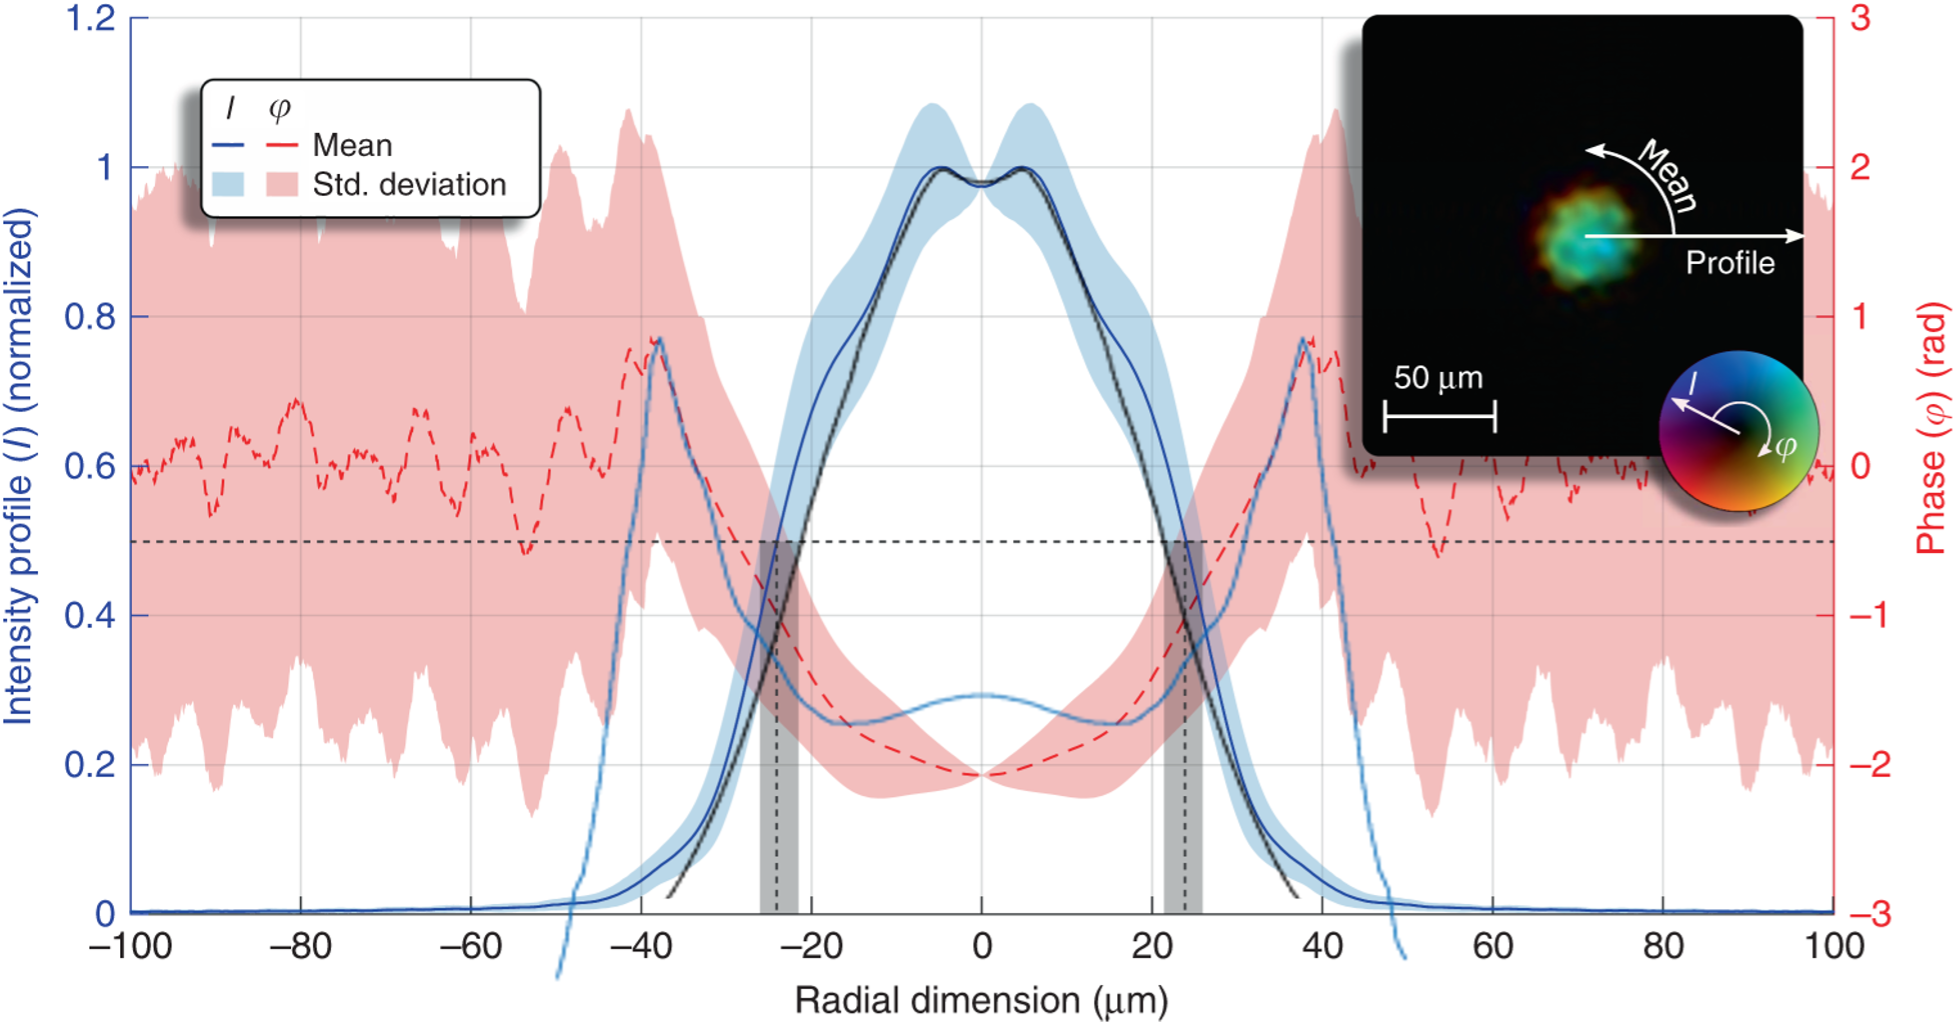
\includegraphics[width=0.74\textwidth]{Figuras/anx_cmp_26.png}
  \caption*{Comparación entre los perfiles radiales de intensidad--fase con $z_{0i}=\qty{3}{mm}$, manteniendo los valores de los parámetros $r_{i,min}=\qty{5}{µm}$, $r_{i,max}=\qty{5}{µm}$ y $k_{i}=\qty{50e6}{m^{-1}}$; y el experimento.}
\end{figure}

\begin{figure}[htbp]
  \centering
  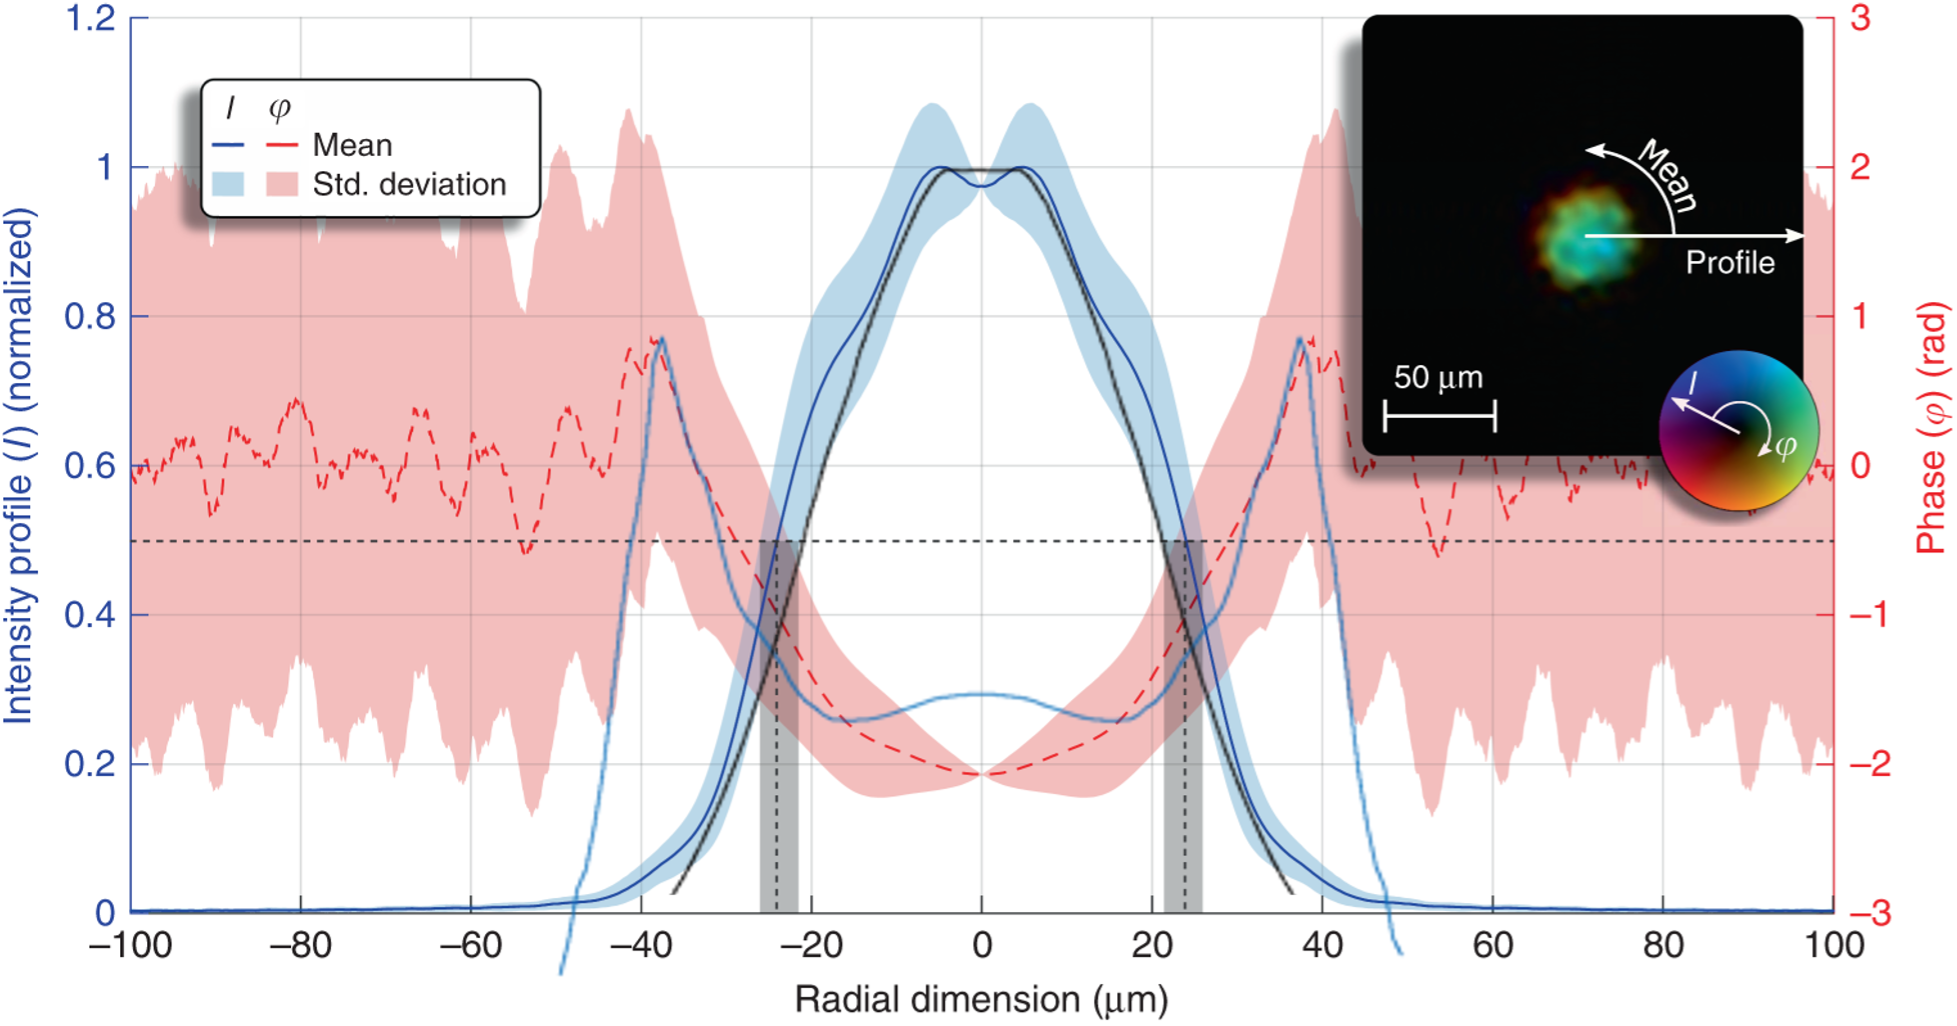
\includegraphics[width=0.74\textwidth]{Figuras/anx_cmp_27.png}
  \caption*{Comparación entre los perfiles radiales de intensidad--fase con $z_{0i}=\qty{3.5}{mm}$, manteniendo los valores de los parámetros $r_{i,min}=\qty{0}{µm}$, $r_{i,max}=\qty{5}{µm}$ y $k_{i}=\qty{50e6}{m^{-1}}$; y el experimento.}
\end{figure}

\begin{figure}[htbp]
  \centering
  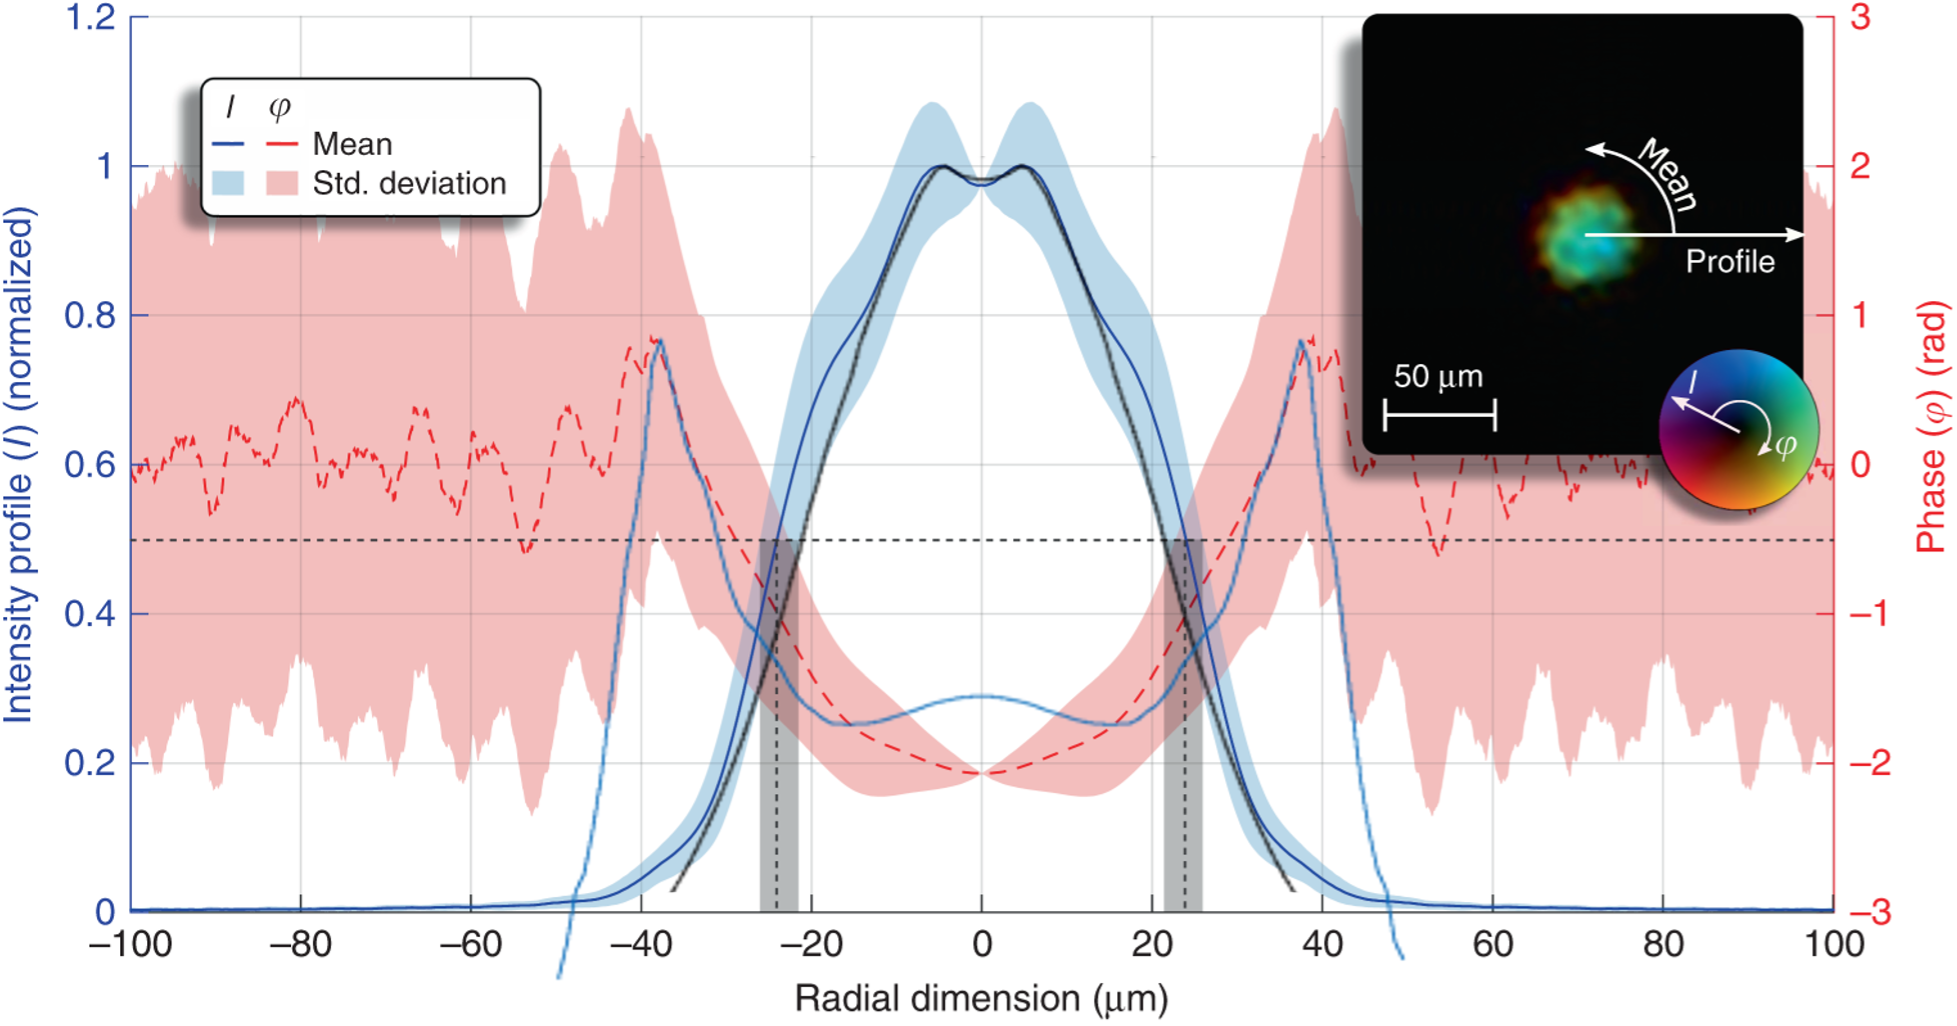
\includegraphics[width=0.74\textwidth]{Figuras/anx_cmp_28.png}
  \caption*{Comparación entre los perfiles radiales de intensidad--fase con $z_{0i}=\qty{3.5}{mm}$, manteniendo los valores de los parámetros $r_{i,min}=\qty{5}{µm}$, $r_{i,max}=\qty{5}{µm}$ y $k_{i}=\qty{50e6}{m^{-1}}$; y el experimento.}
\end{figure}

\subsection*{Variando el parámetro $k_{i}$}

\begin{figure}[htbp]
  \centering
  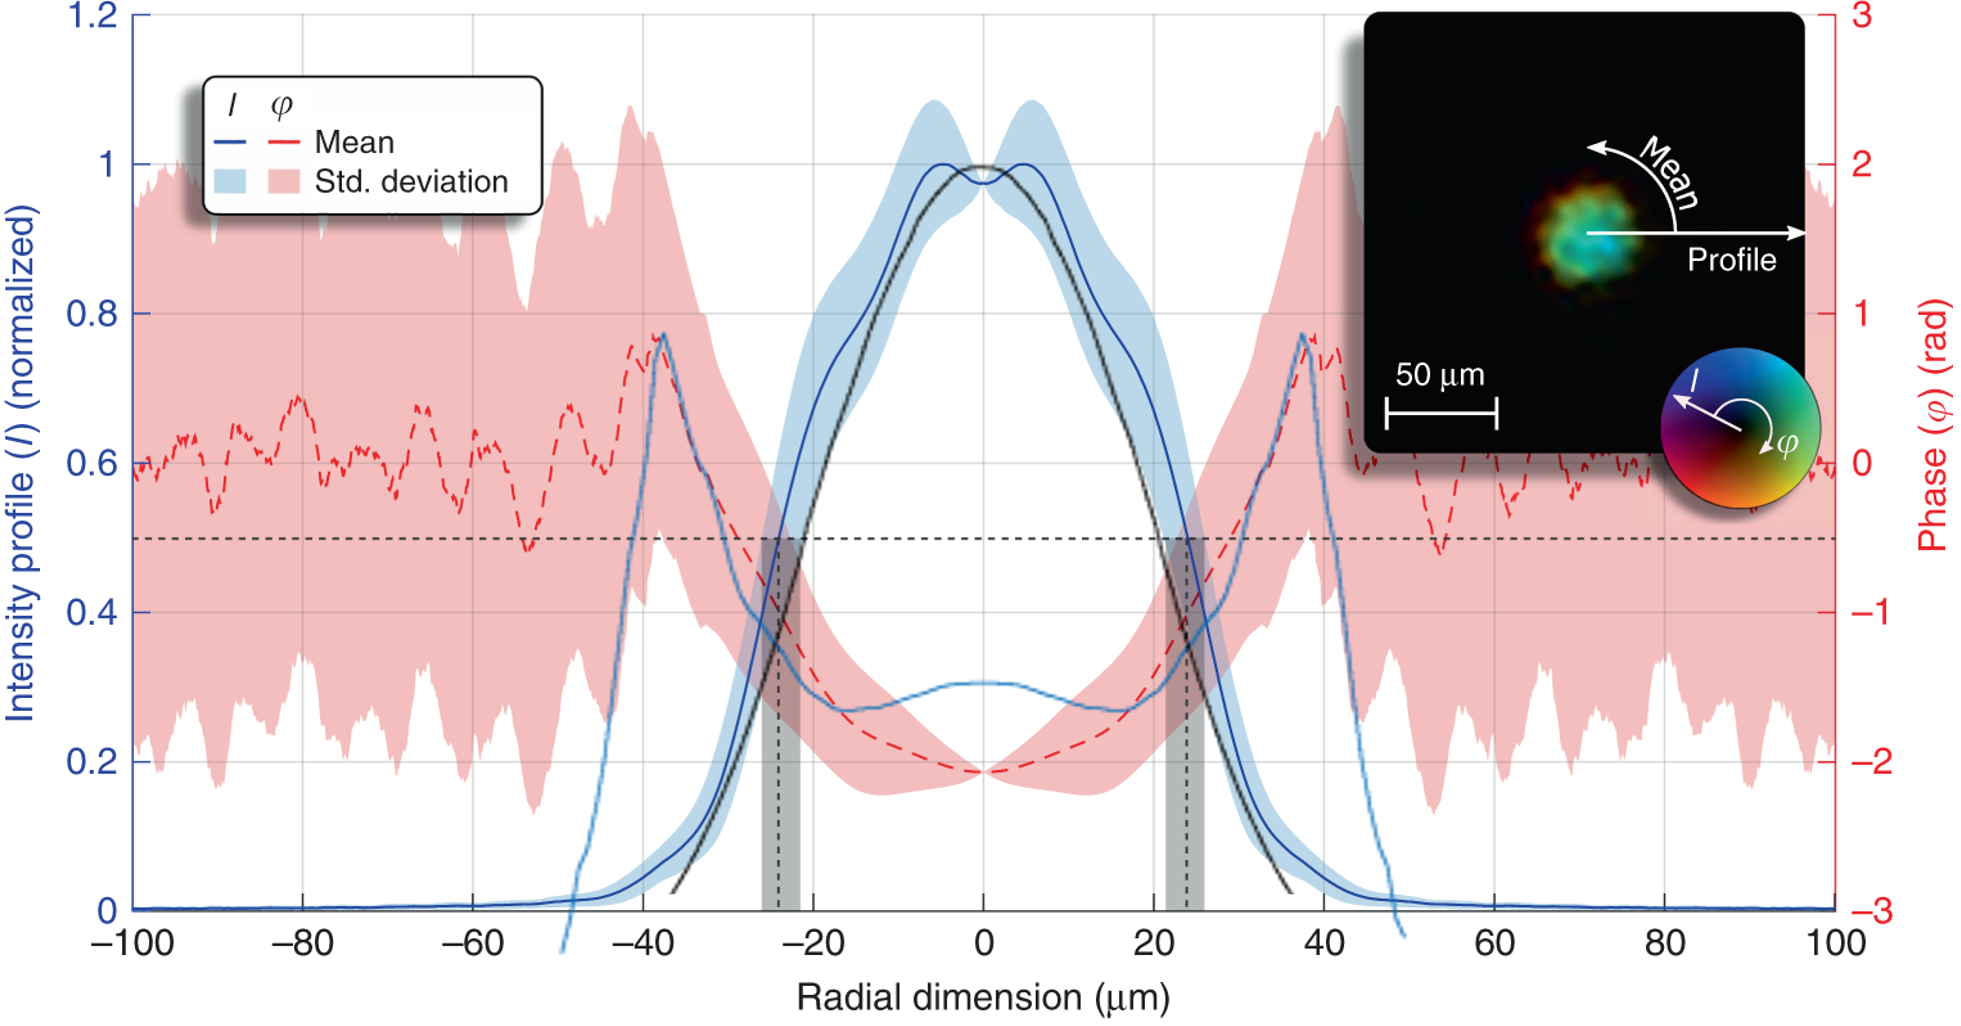
\includegraphics[width=0.74\textwidth]{Figuras/anx_cmp_31.png}
  \caption*{Comparación entre los perfiles radiales de intensidad--fase con $z_{0i}=\qty{2}{mm}$ y $k_{i}=\qty{2000}{m^{-1}}$, manteniendo los valores de los parámetros $r_{i,min}=\qty{0}{µm}$ y $r_{i,max}=\qty{5}{µm}$; y el experimento.}
\end{figure}

\begin{figure}[htbp!]
  \centering
  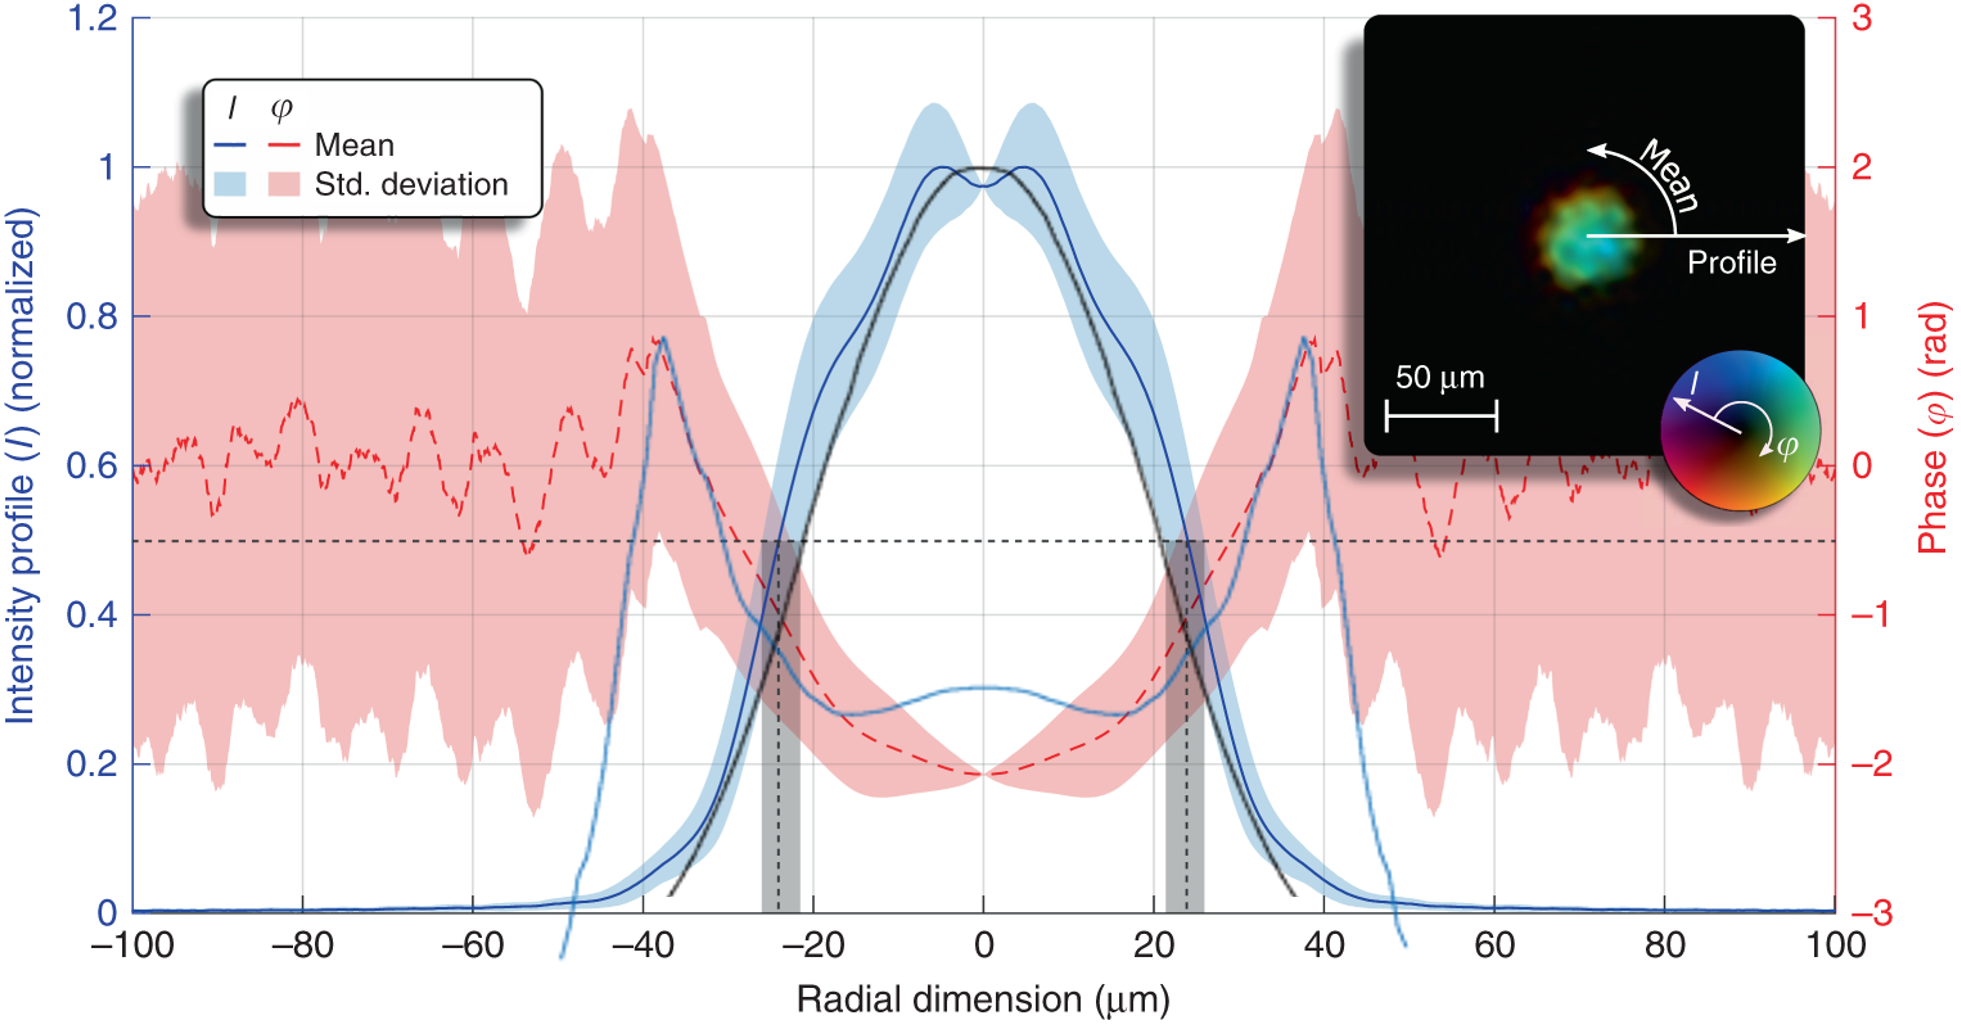
\includegraphics[width=0.74\textwidth]{Figuras/anx_cmp_32.png}
  \caption*{Comparación entre los perfiles radiales de intensidad--fase con $z_{0i}=\qty{2.5}{mm}$ y $k_{i}=\qty{2500}{m^{-1}}$, manteniendo los valores de los parámetros $r_{i,min}=\qty{0}{µm}$ y $r_{i,max}=\qty{5}{µm}$; y el experimento.}
\end{figure}

\begin{figure}[htbp!]
  \centering
  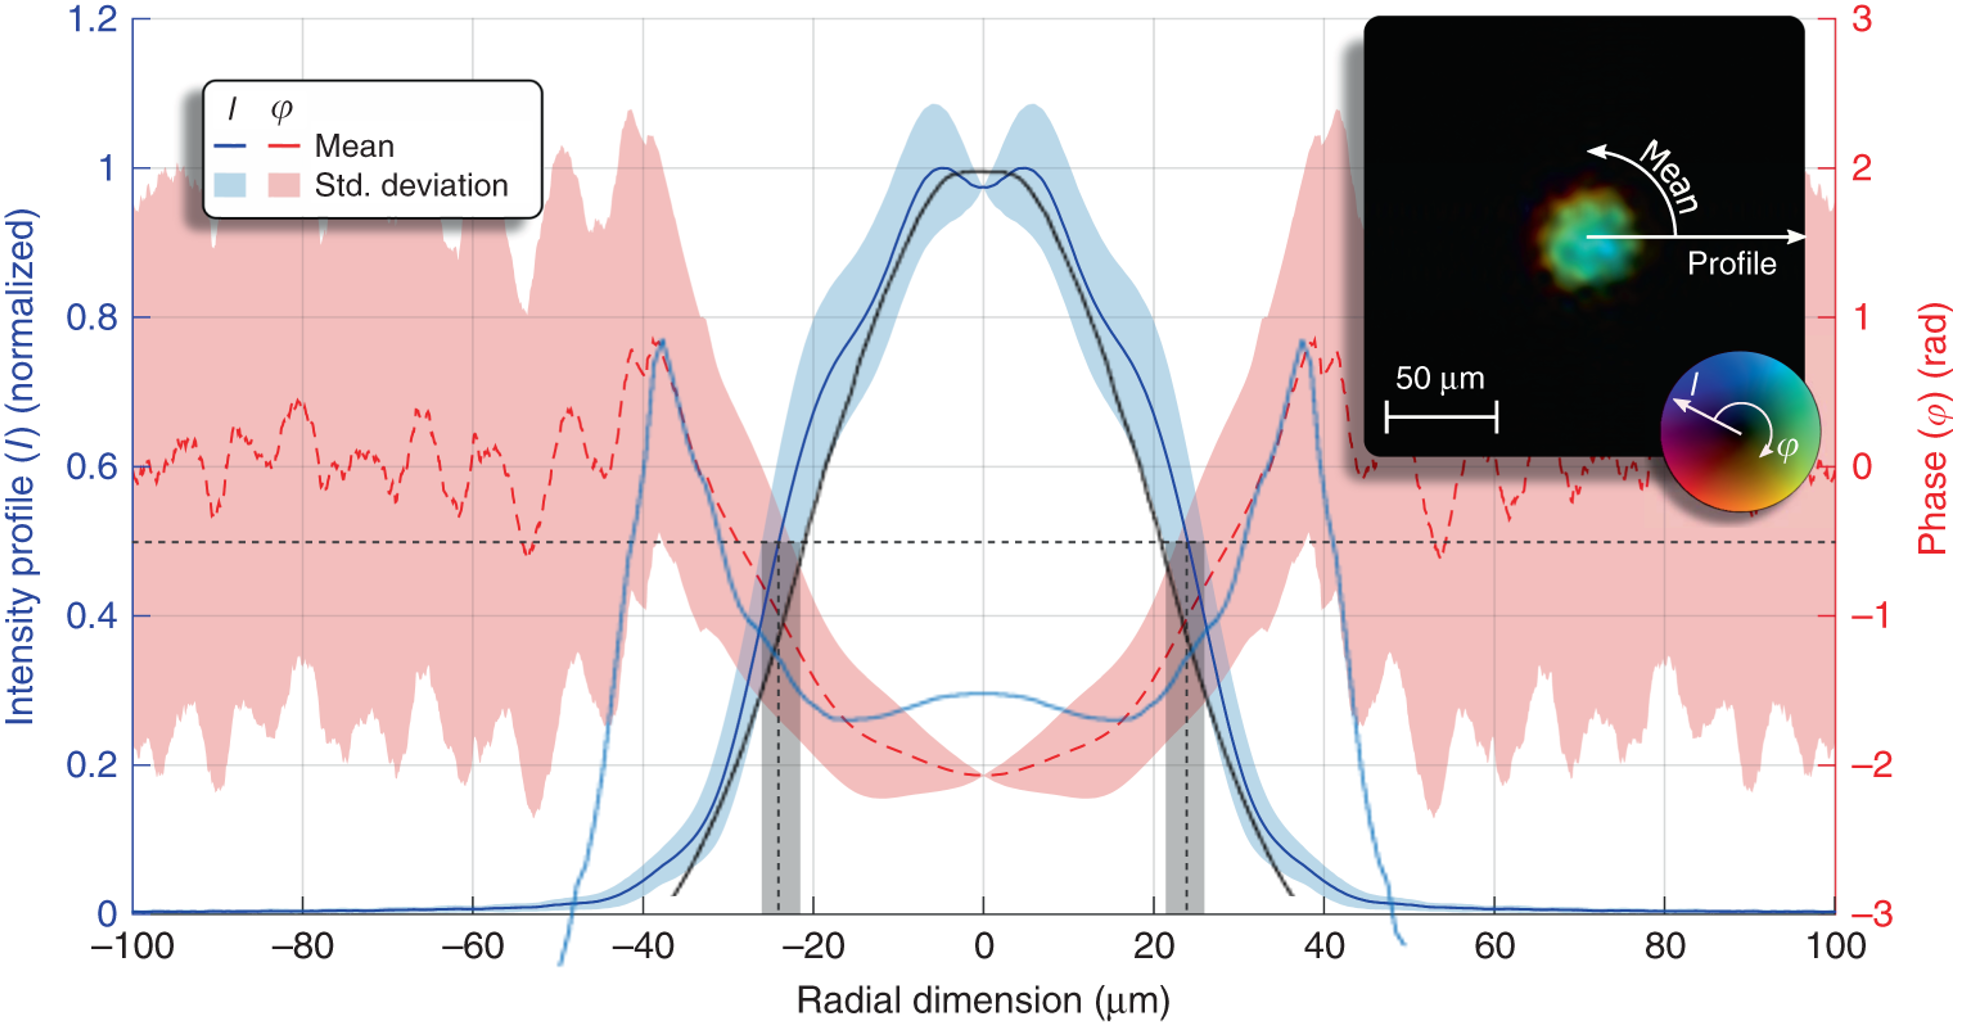
\includegraphics[width=0.74\textwidth]{Figuras/anx_cmp_33.png}
  \caption*{Comparación entre los perfiles radiales de intensidad--fase con $z_{0i}=\qty{3}{mm}$ y $k_{i}=\qty{3000}{m^{-1}}$, manteniendo los valores de los parámetros $r_{i,min}=\qty{0}{µm}$ y $r_{i,max}=\qty{5}{µm}$; y el experimento.}
\end{figure}

\begin{figure}[htbp]
  \centering
  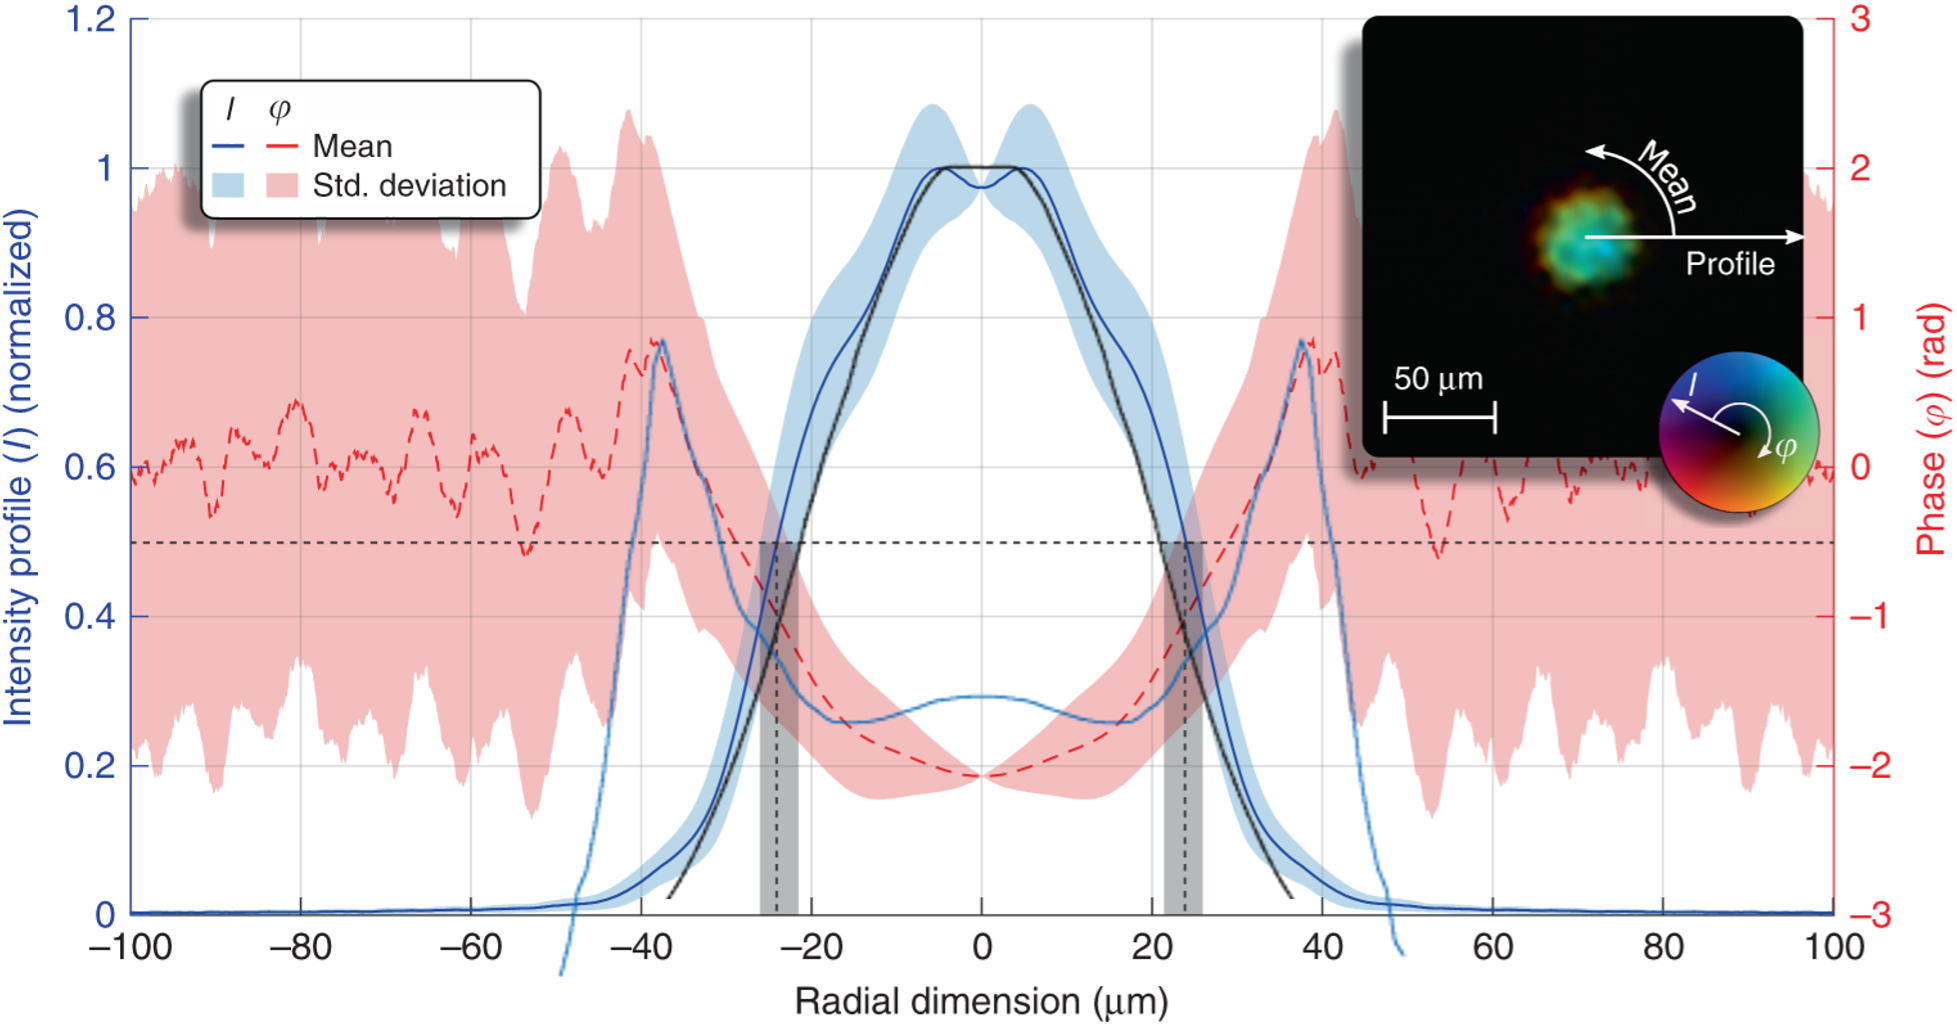
\includegraphics[width=0.7\textwidth]{Figuras/anx_cmp_34.png}
  \caption*{Comparación entre los perfiles radiales de intensidad--fase con $z_{0i}=\qty{3.5}{mm}$ y $k_{i}=\qty{4000}{m^{-1}}$, manteniendo los valores de los parámetros $r_{i,min}=\qty{0}{µm}$ y $r_{i,max}=\qty{5}{µm}$; y el experimento.}
\end{figure}

\subsection*{Variando el parámetro \texttt{zshift}}

\begin{figure}[htbp]
  \centering
  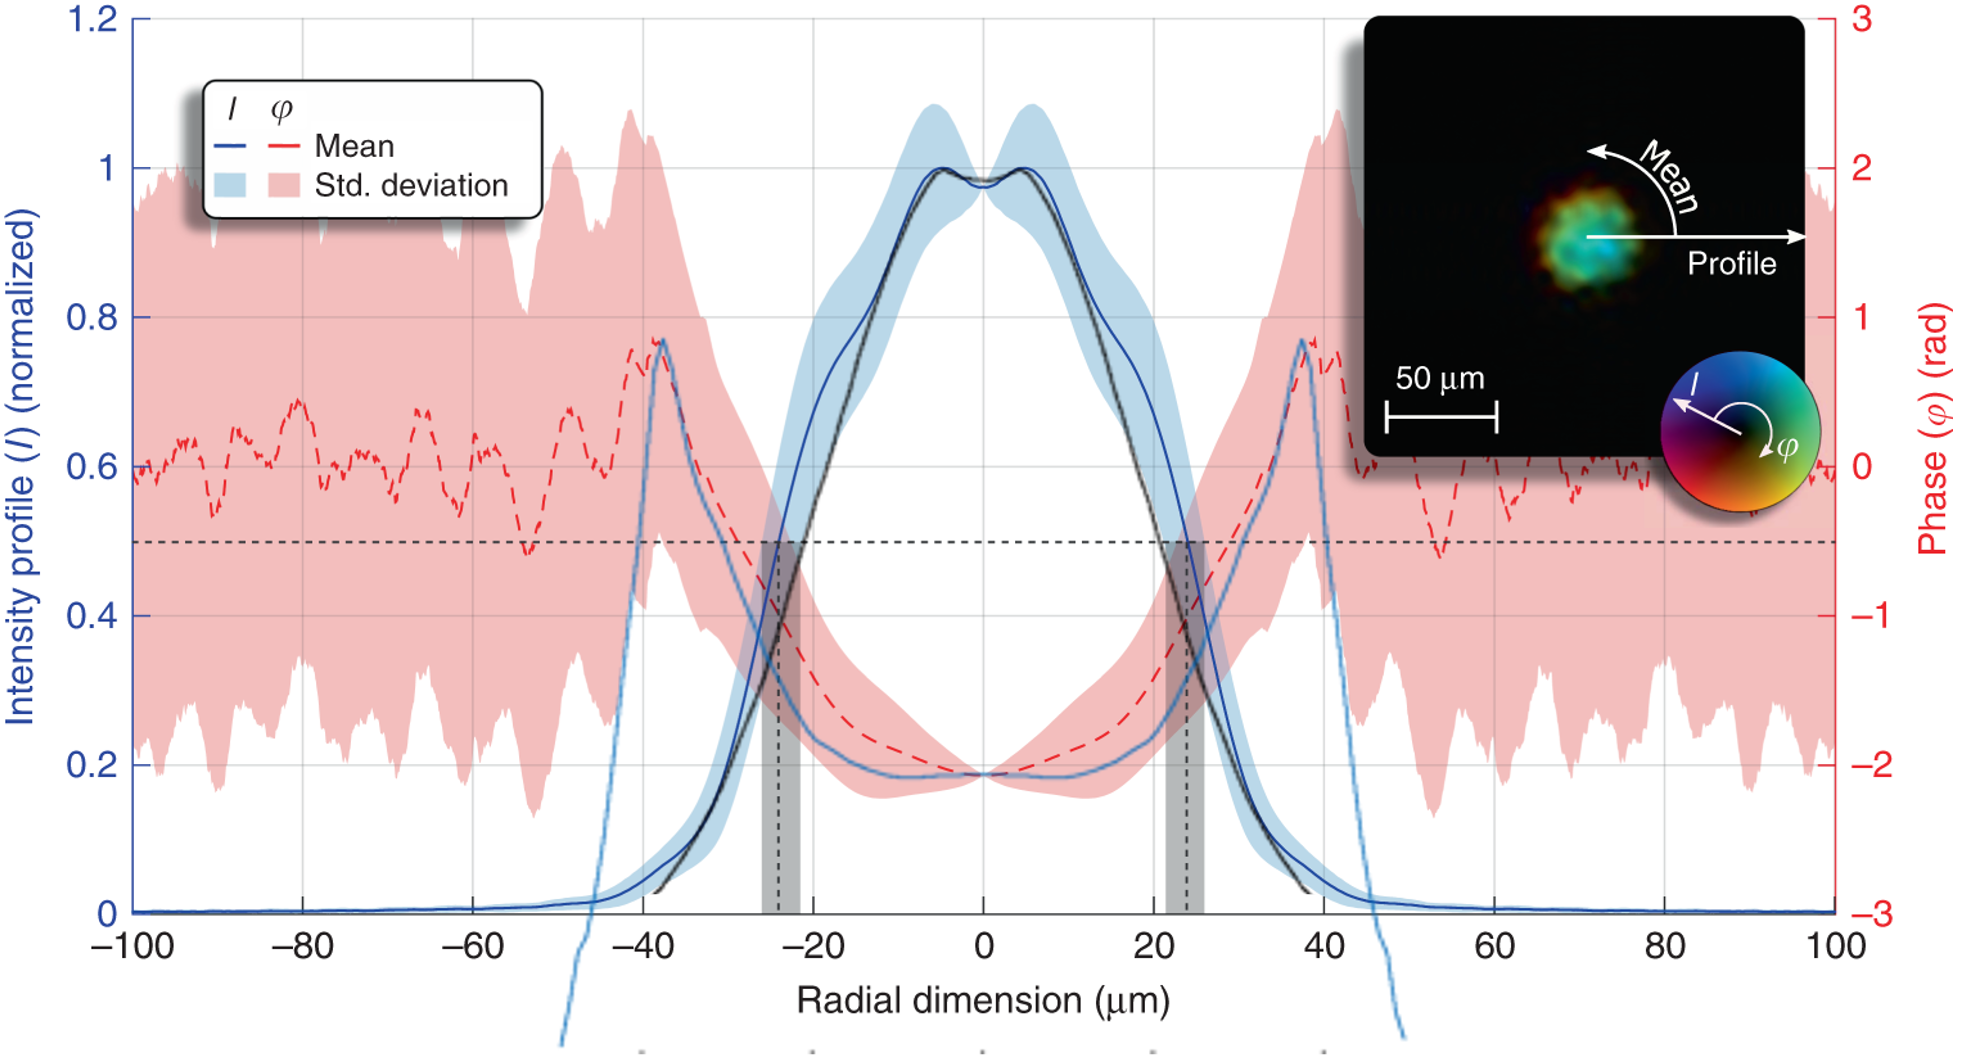
\includegraphics[width=0.7\textwidth]{Figuras/anx_cmp_41.png}
  \caption*{Comparación entre los perfiles radiales de intensidad--fase con $r_{i,min}=r_{i,max}=\qty{5}{µm}$ y $\texttt{zshift}=0.55$; manteniendo los valores de los parámetros $k_{i}=\qty{50e6}{m^{-1}}$ y $z_{0i}=\qty{3.5}{mm}$; y el experimento.}
\end{figure}

\begin{figure}[htbp!]
  \centering
  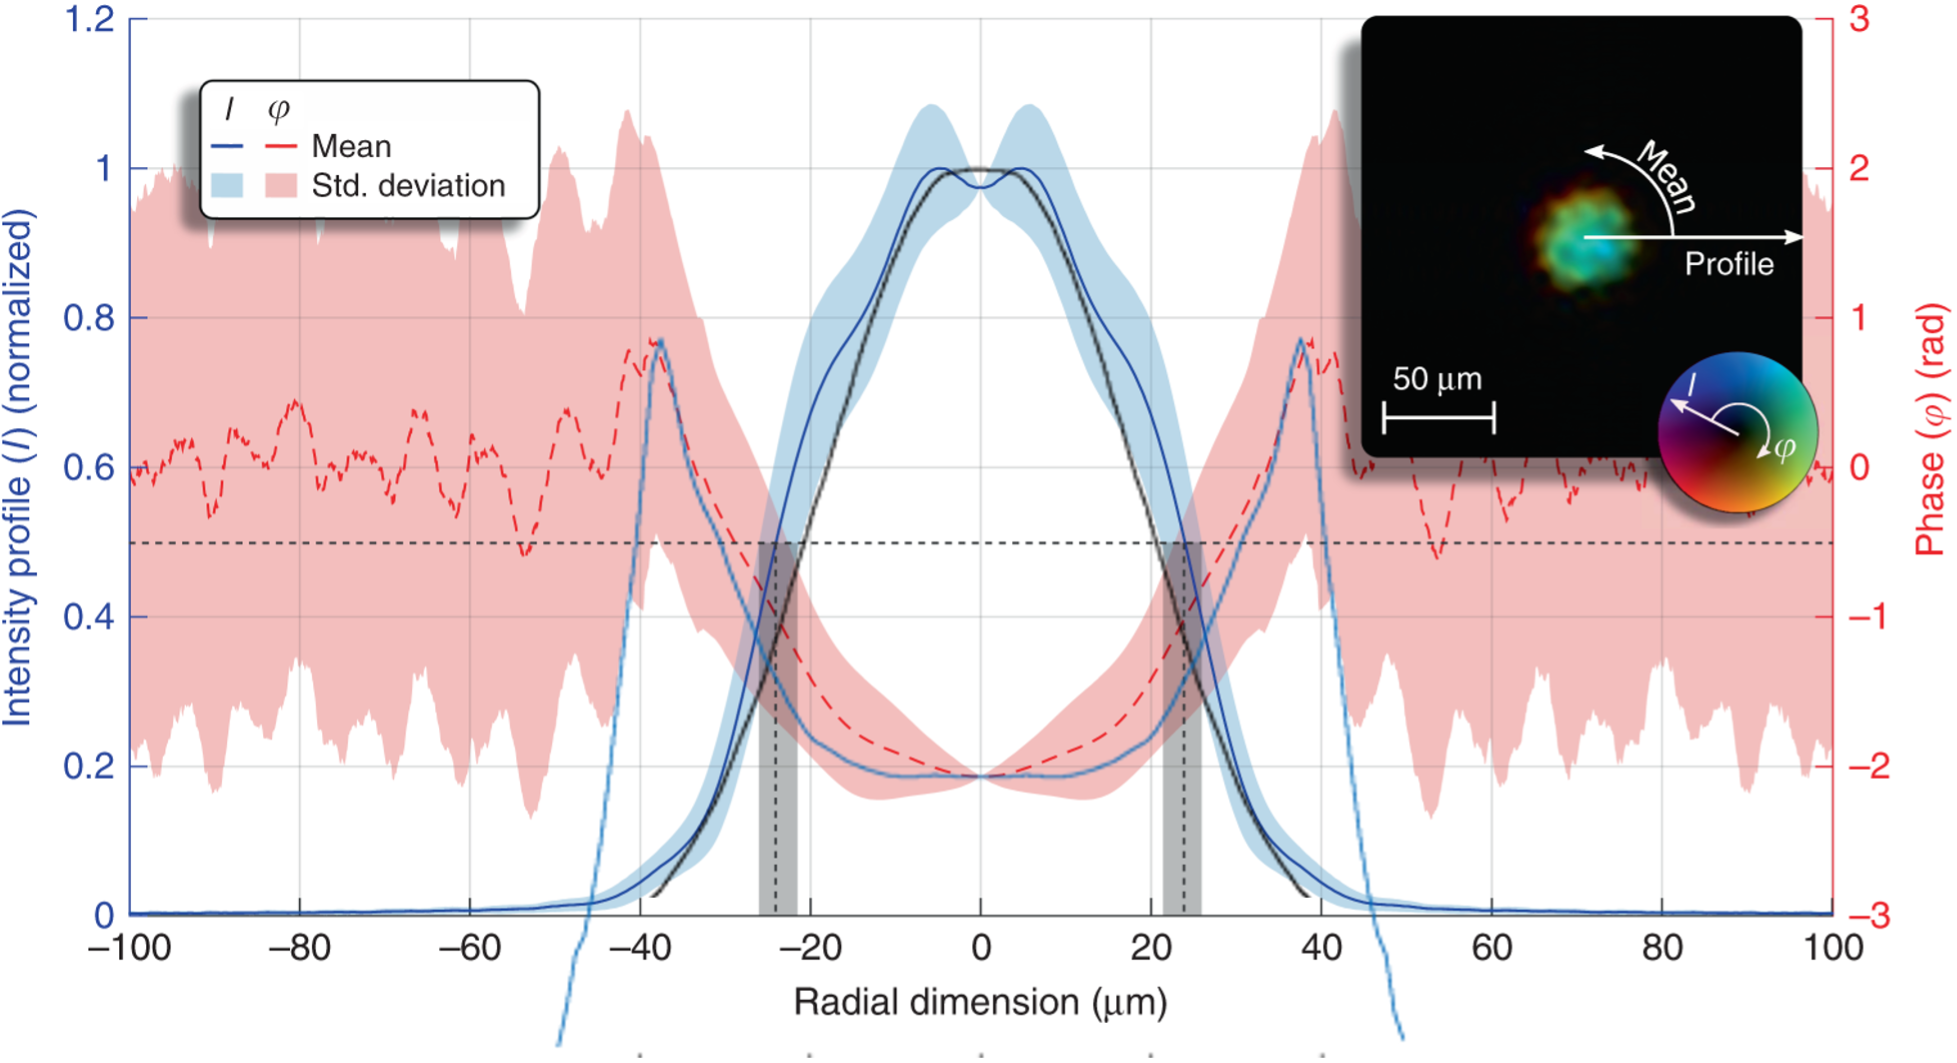
\includegraphics[width=0.7\textwidth]{Figuras/anx_cmp_42.png}
  \caption*{Comparación entre los perfiles radiales de intensidad--fase con $r_{i,min}=\qty{0}{µm}$, $r_{i,max}=\qty{5}{µm}$ y $\texttt{zshift}=0.55$; manteniendo los valores de los parámetros $k_{i}=\qty{50e6}{m^{-1}}$ y $z_{0i}=\qty{3.5}{mm}$; y el experimento.}
\end{figure}

\begin{figure}[htbp]
  \centering
  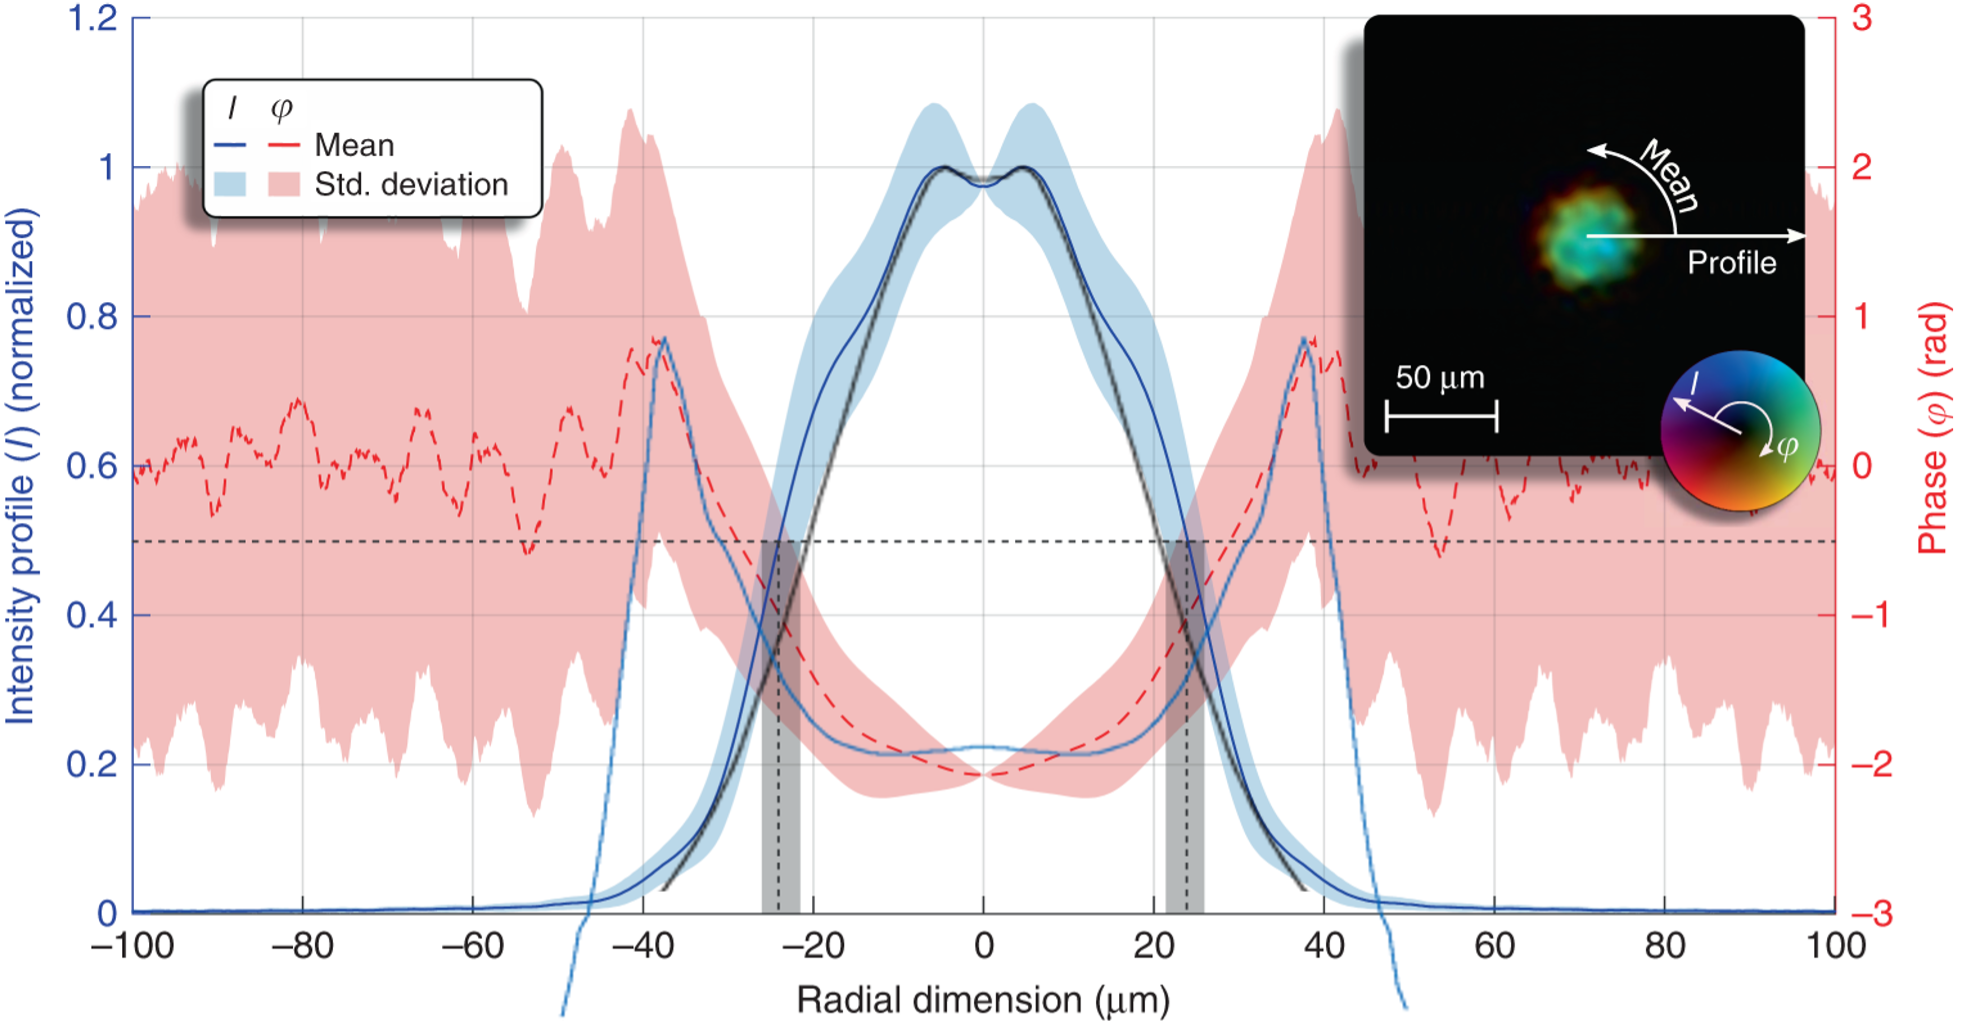
\includegraphics[width=0.7\textwidth]{Figuras/anx_cmp_43.png}
  \caption*{Comparación entre los perfiles radiales de intensidad--fase con $r_{i,min}=r_{i,max}=\qty{5}{µm}$ y $\texttt{zshift}=0.6$; manteniendo los valores de los parámetros $k_{i}=\qty{50e6}{m^{-1}}$ y $z_{0i}=\qty{3.5}{mm}$; y el experimento.}
\end{figure}

\begin{figure}[htbp]
  \centering
  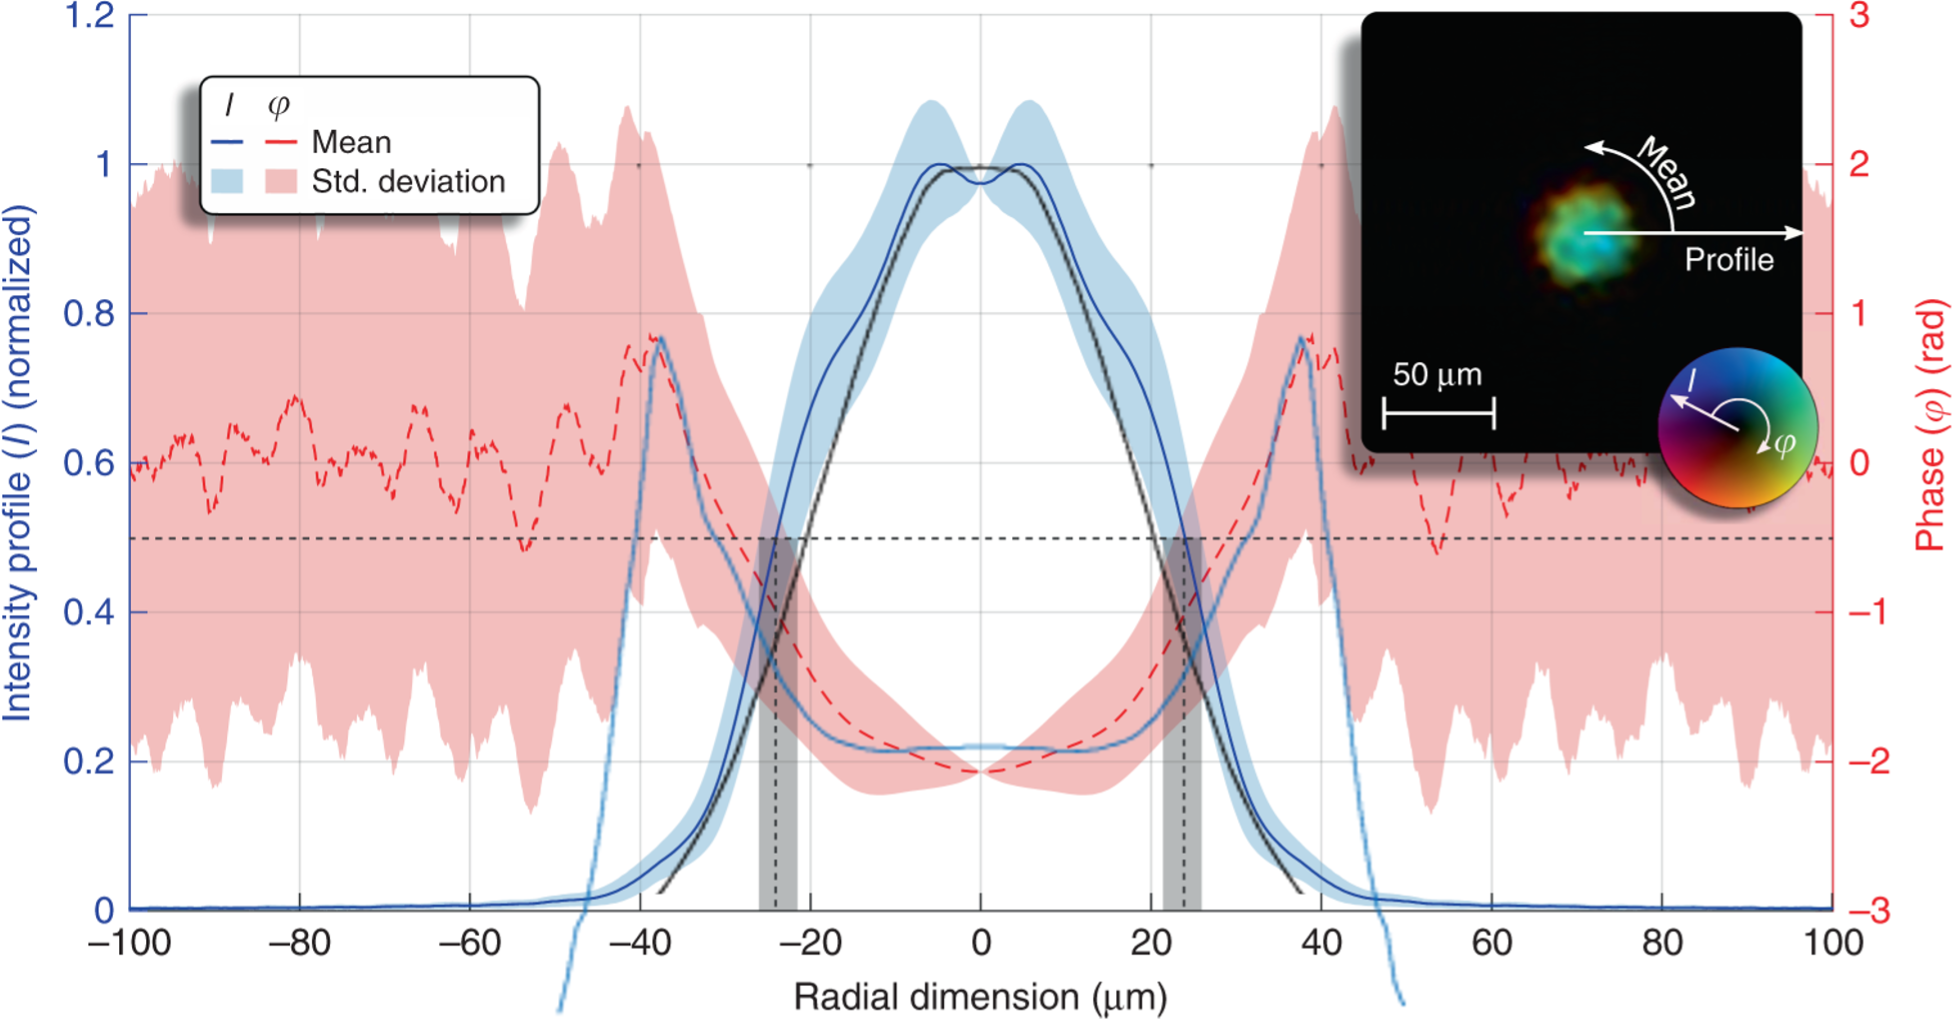
\includegraphics[width=0.7\textwidth]{Figuras/anx_cmp_44.png}
  \caption*{Comparación entre los perfiles radiales de intensidad--fase con $r_{i,min}=\qty{0}{µm}$, $r_{i,max}=\qty{5}{µm}$ y $\texttt{zshift}=0.6$; manteniendo los valores de los parámetros $k_{i}=\qty{50e6}{m^{-1}}$ y $z_{0i}=\qty{3.5}{mm}$; y el experimento.}
\end{figure}

\begin{figure}[htbp]
  \centering
  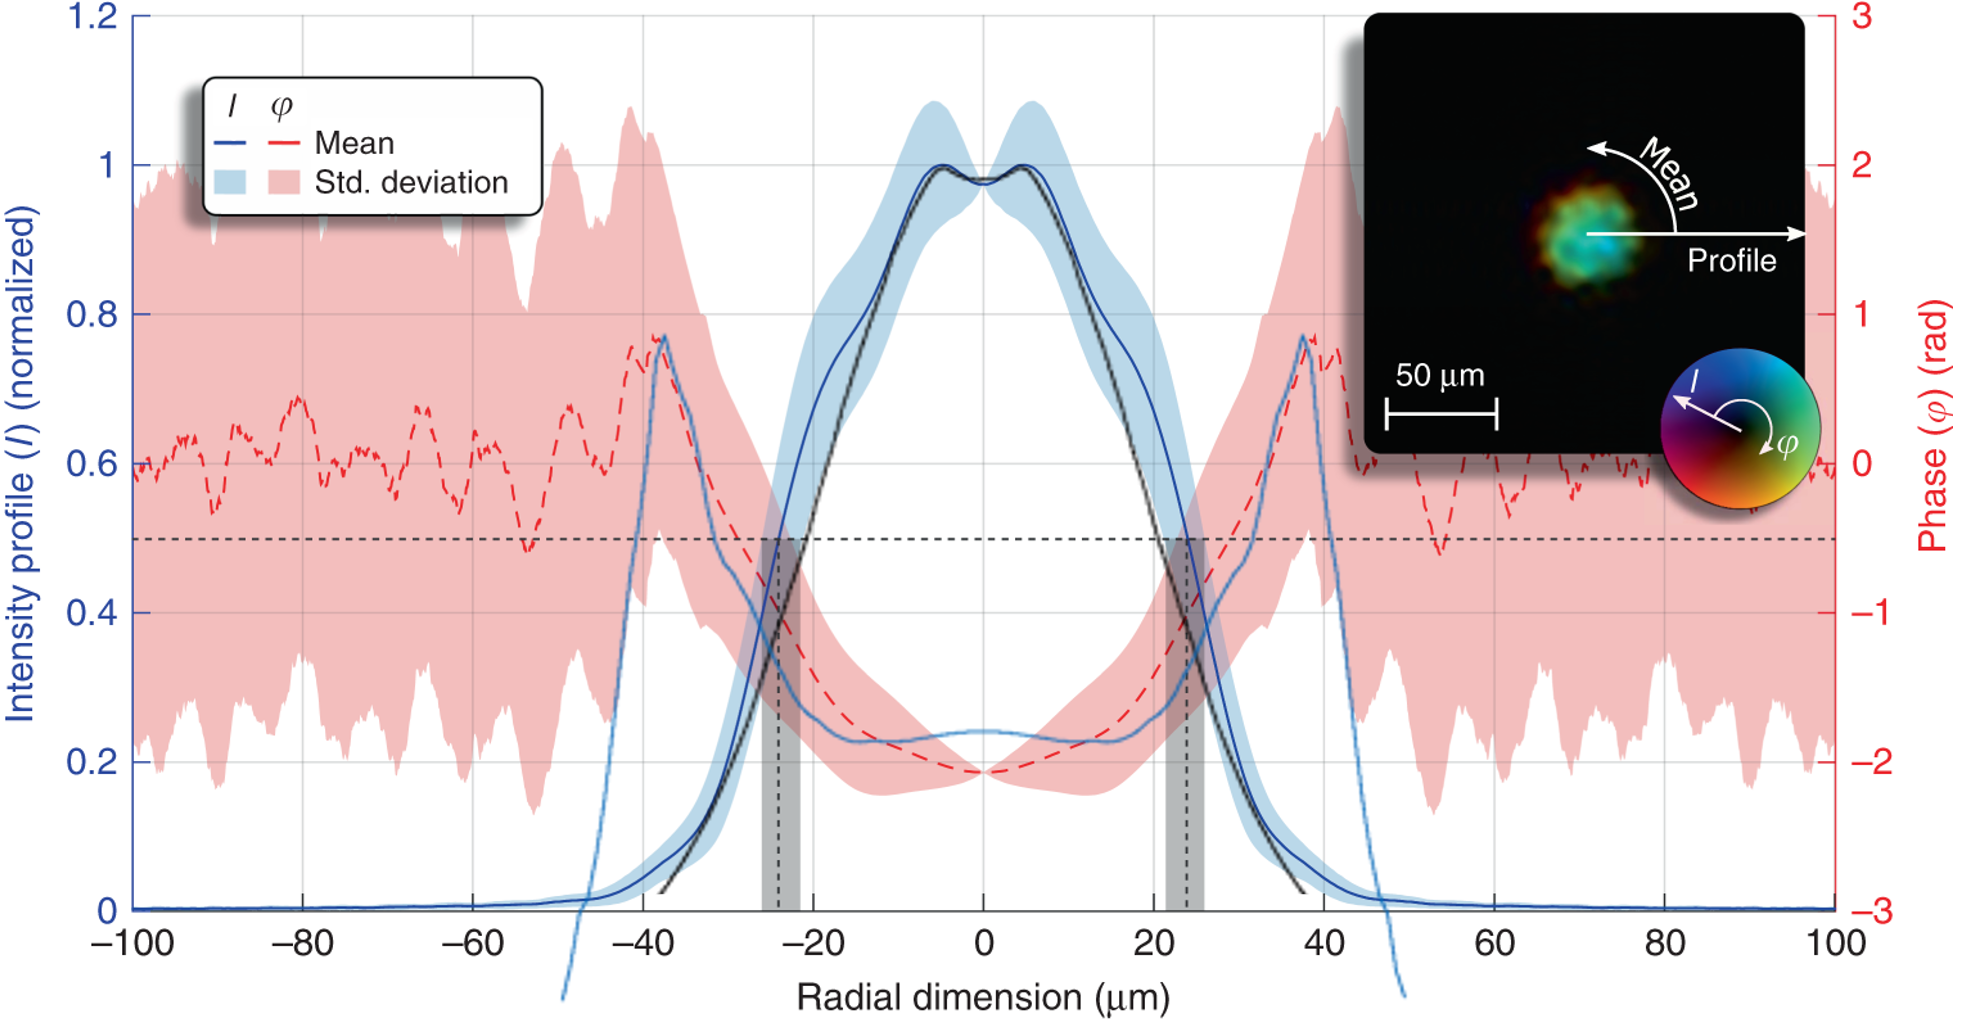
\includegraphics[width=0.7\textwidth]{Figuras/anx_cmp_45.png}
  \caption*{Comparación entre los perfiles radiales de intensidad--fase con $r_{i,min}=r_{i,max}=\qty{5}{µm}$ y $\texttt{zshift}=0.65$; manteniendo los valores de los parámetros $k_{i}=\qty{50e6}{m^{-1}}$ y $z_{0i}=\qty{3.5}{mm}$; y el experimento.}
\end{figure}

\begin{figure}[htbp]
  \centering
  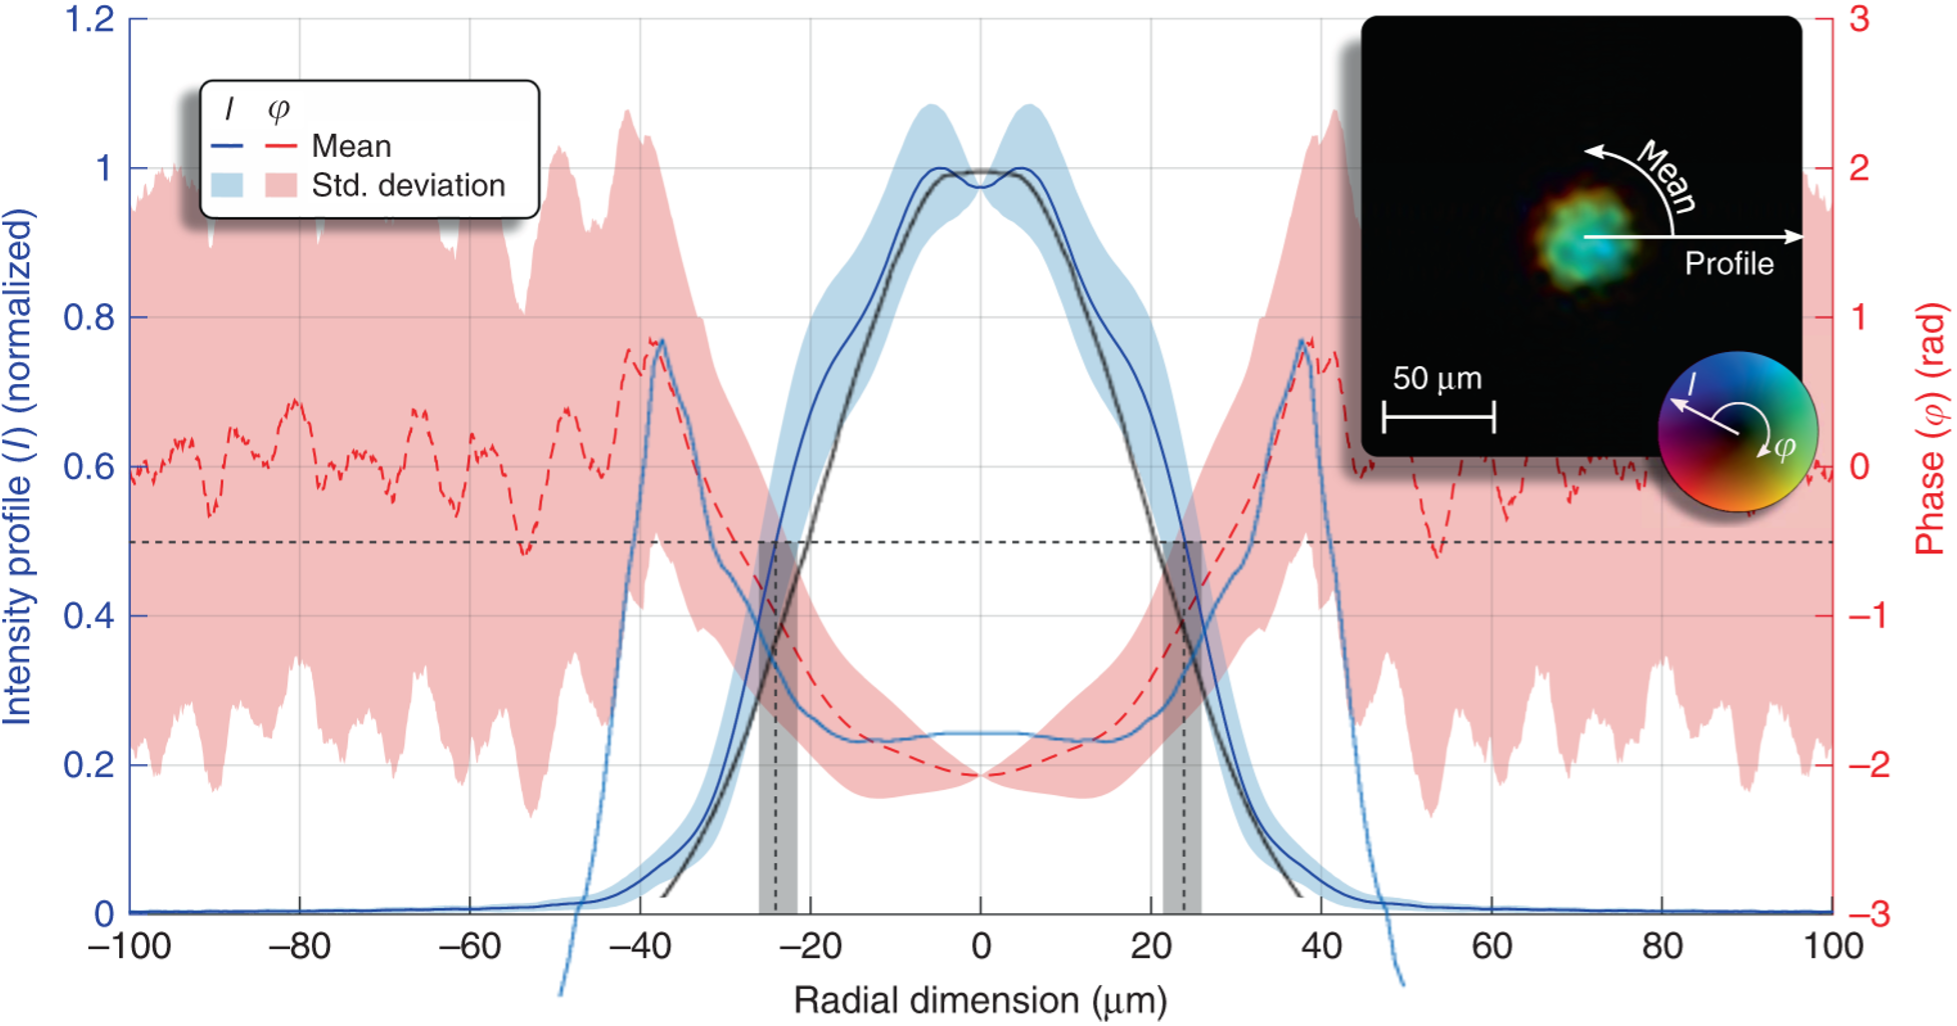
\includegraphics[width=0.7\textwidth]{Figuras/anx_cmp_46.png}
  \caption*{Comparación entre los perfiles radiales de intensidad--fase con $r_{i,min}=\qty{0}{µm}$, $r_{i,max}=\qty{5}{µm}$ y $\texttt{zshift}=0.65$; manteniendo los valores de los parámetros $k_{i}=\qty{50e6}{m^{-1}}$ y $z_{0i}=\qty{3.5}{mm}$; y el experimento.}
\end{figure}

\begin{figure}[htbp]
  \centering
  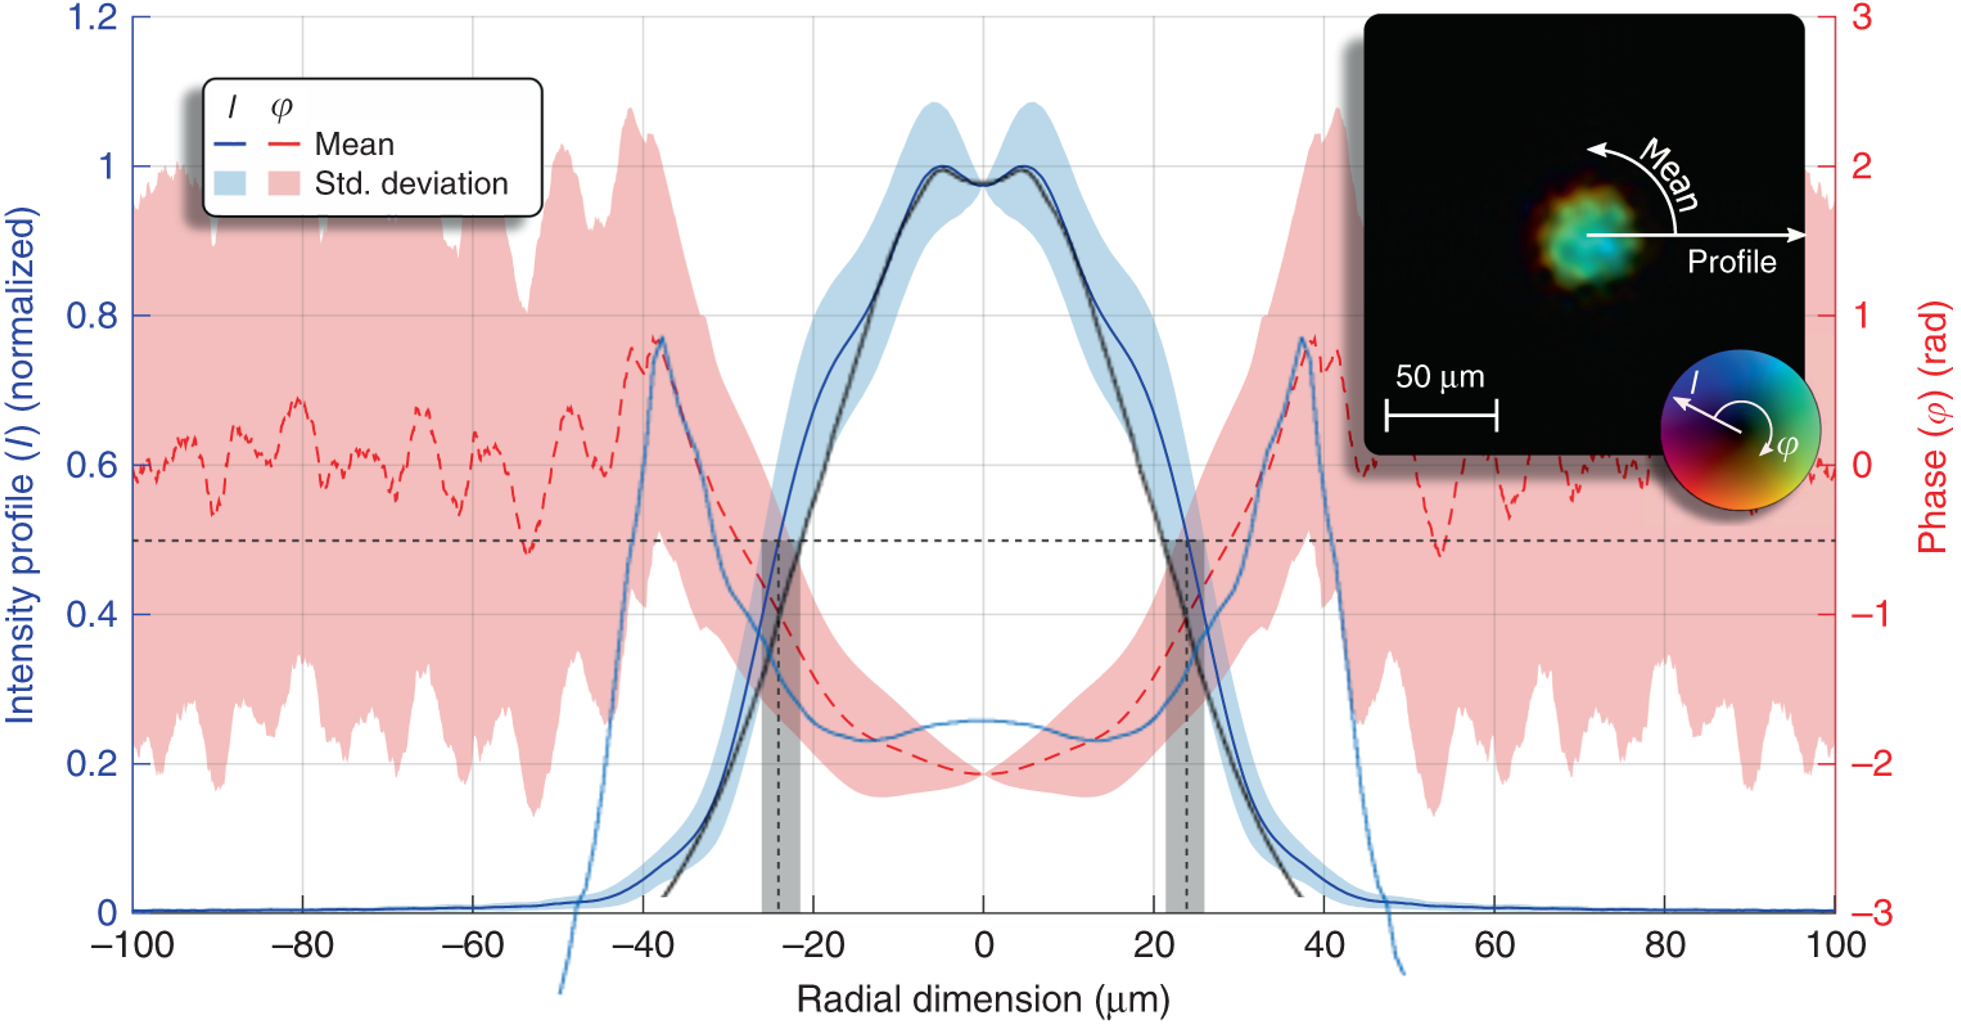
\includegraphics[width=0.7\textwidth]{Figuras/anx_cmp_47.png}
  \caption*{Comparación entre los perfiles radiales de intensidad--fase con $r_{i,min}=r_{i,max}=\qty{5}{µm}$ y $\texttt{zshift}=0.7$; manteniendo los valores de los parámetros $k_{i}=\qty{50e6}{m^{-1}}$ y $z_{0i}=\qty{3.5}{mm}$; y el experimento.}
\end{figure}

\begin{figure}[htbp]
  \centering
  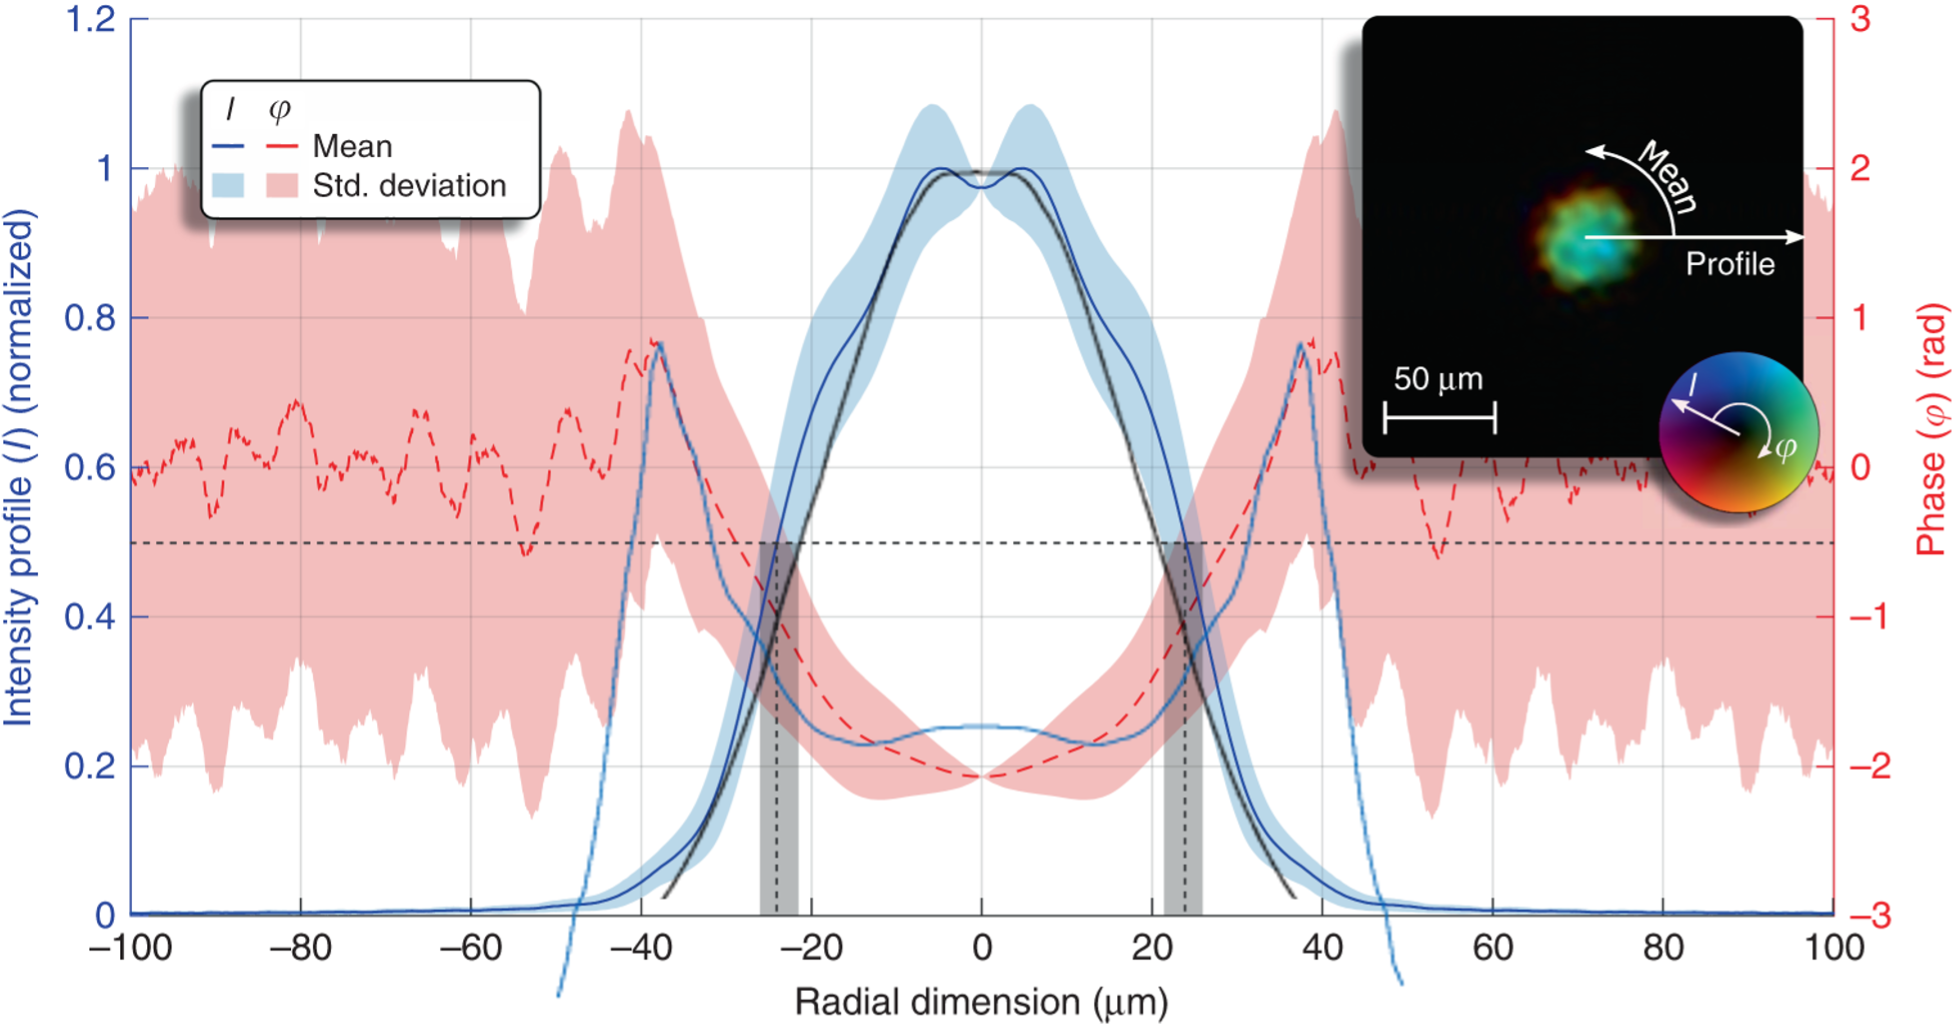
\includegraphics[width=0.7\textwidth]{Figuras/anx_cmp_48.png}
  \caption*{Comparación entre los perfiles radiales de intensidad--fase con $r_{i,min}=\qty{0}{µm}$, $r_{i,max}=\qty{5}{µm}$ y $\texttt{zshift}=0.7$; manteniendo los valores de los parámetros $k_{i}=\qty{50e6}{m^{-1}}$ y $z_{0i}=\qty{3.5}{mm}$; y el experimento.}
\end{figure}

\begin{figure}[htbp]
  \centering
  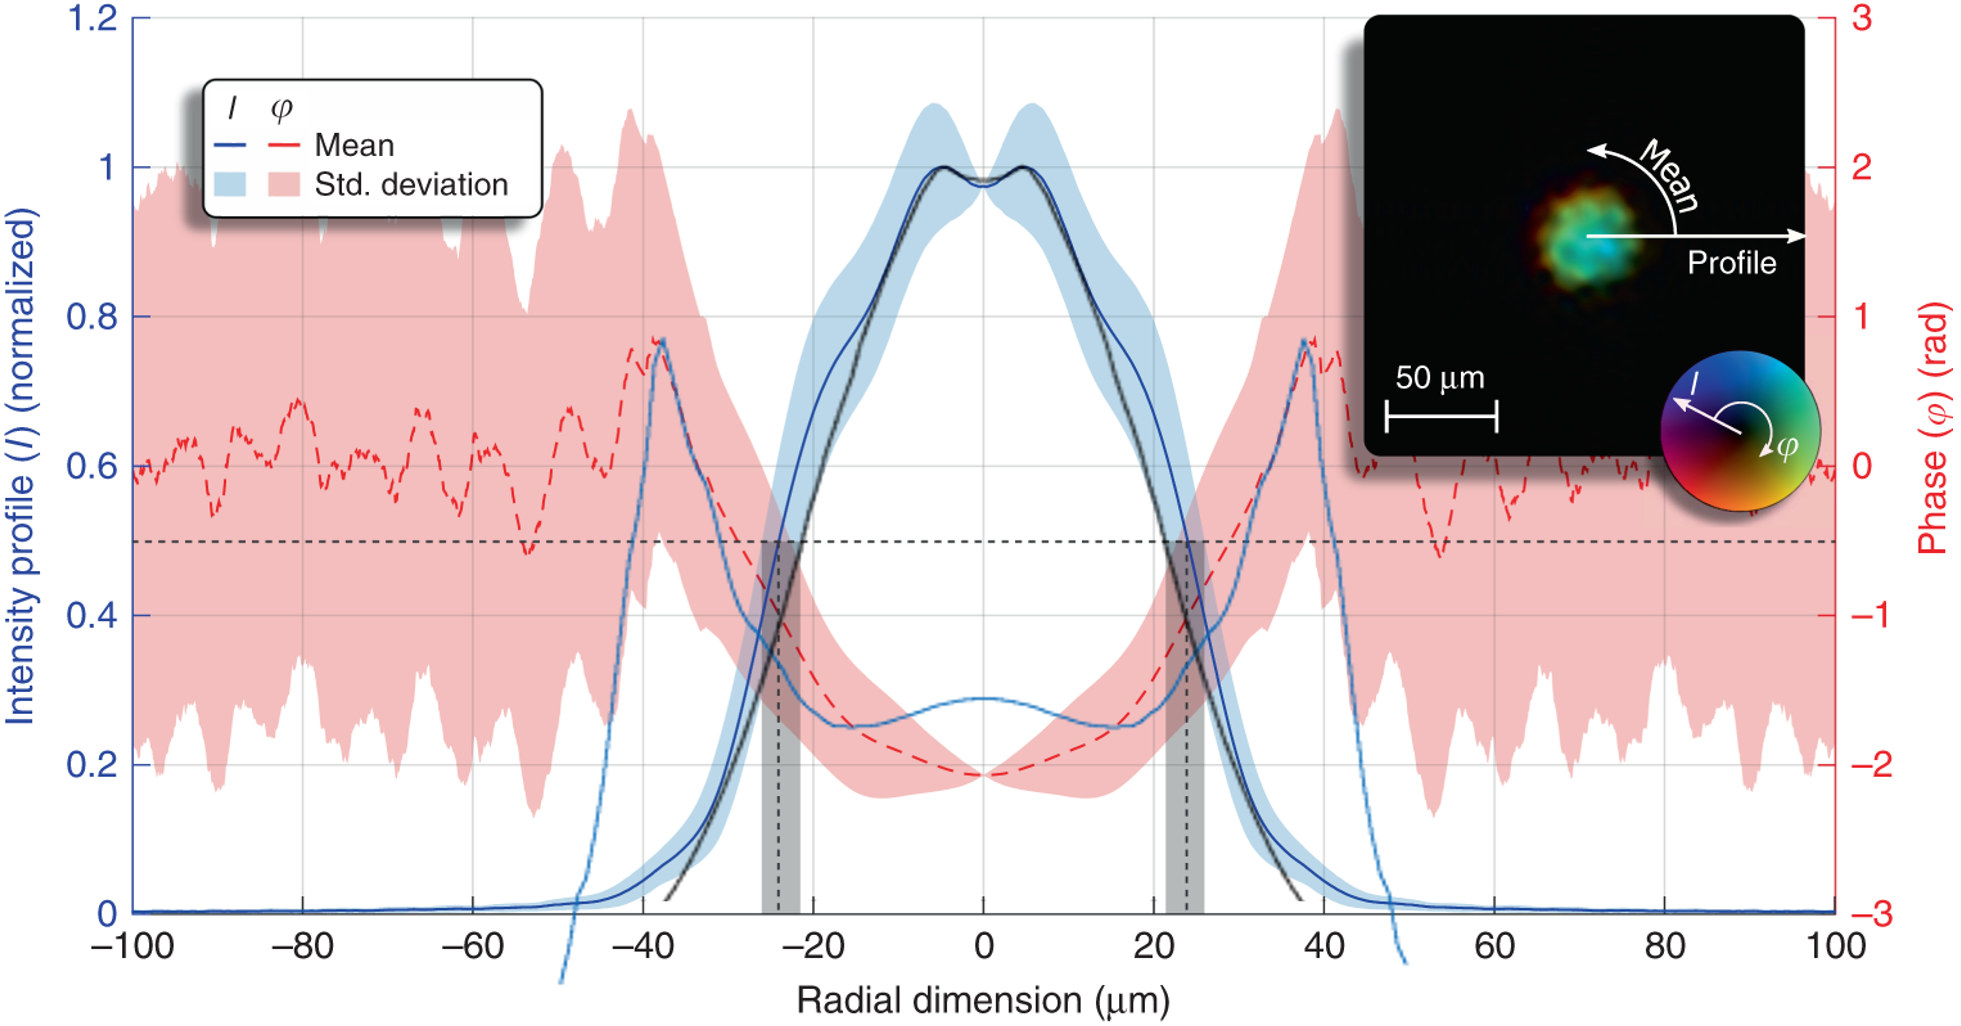
\includegraphics[width=0.75\textwidth]{Figuras/anx_cmp_49.png}
  \caption*{Comparación entre los perfiles radiales de intensidad--fase con $r_{i,min}=r_{i,max}=\qty{5}{µm}$ y $\texttt{zshift}=0.75$; manteniendo los valores de los parámetros $k_{i}=\qty{50e6}{m^{-1}}$ y $z_{0i}=\qty{3.5}{mm}$; y el experimento.}
\end{figure}

\begin{figure}[htbp]
  \centering
  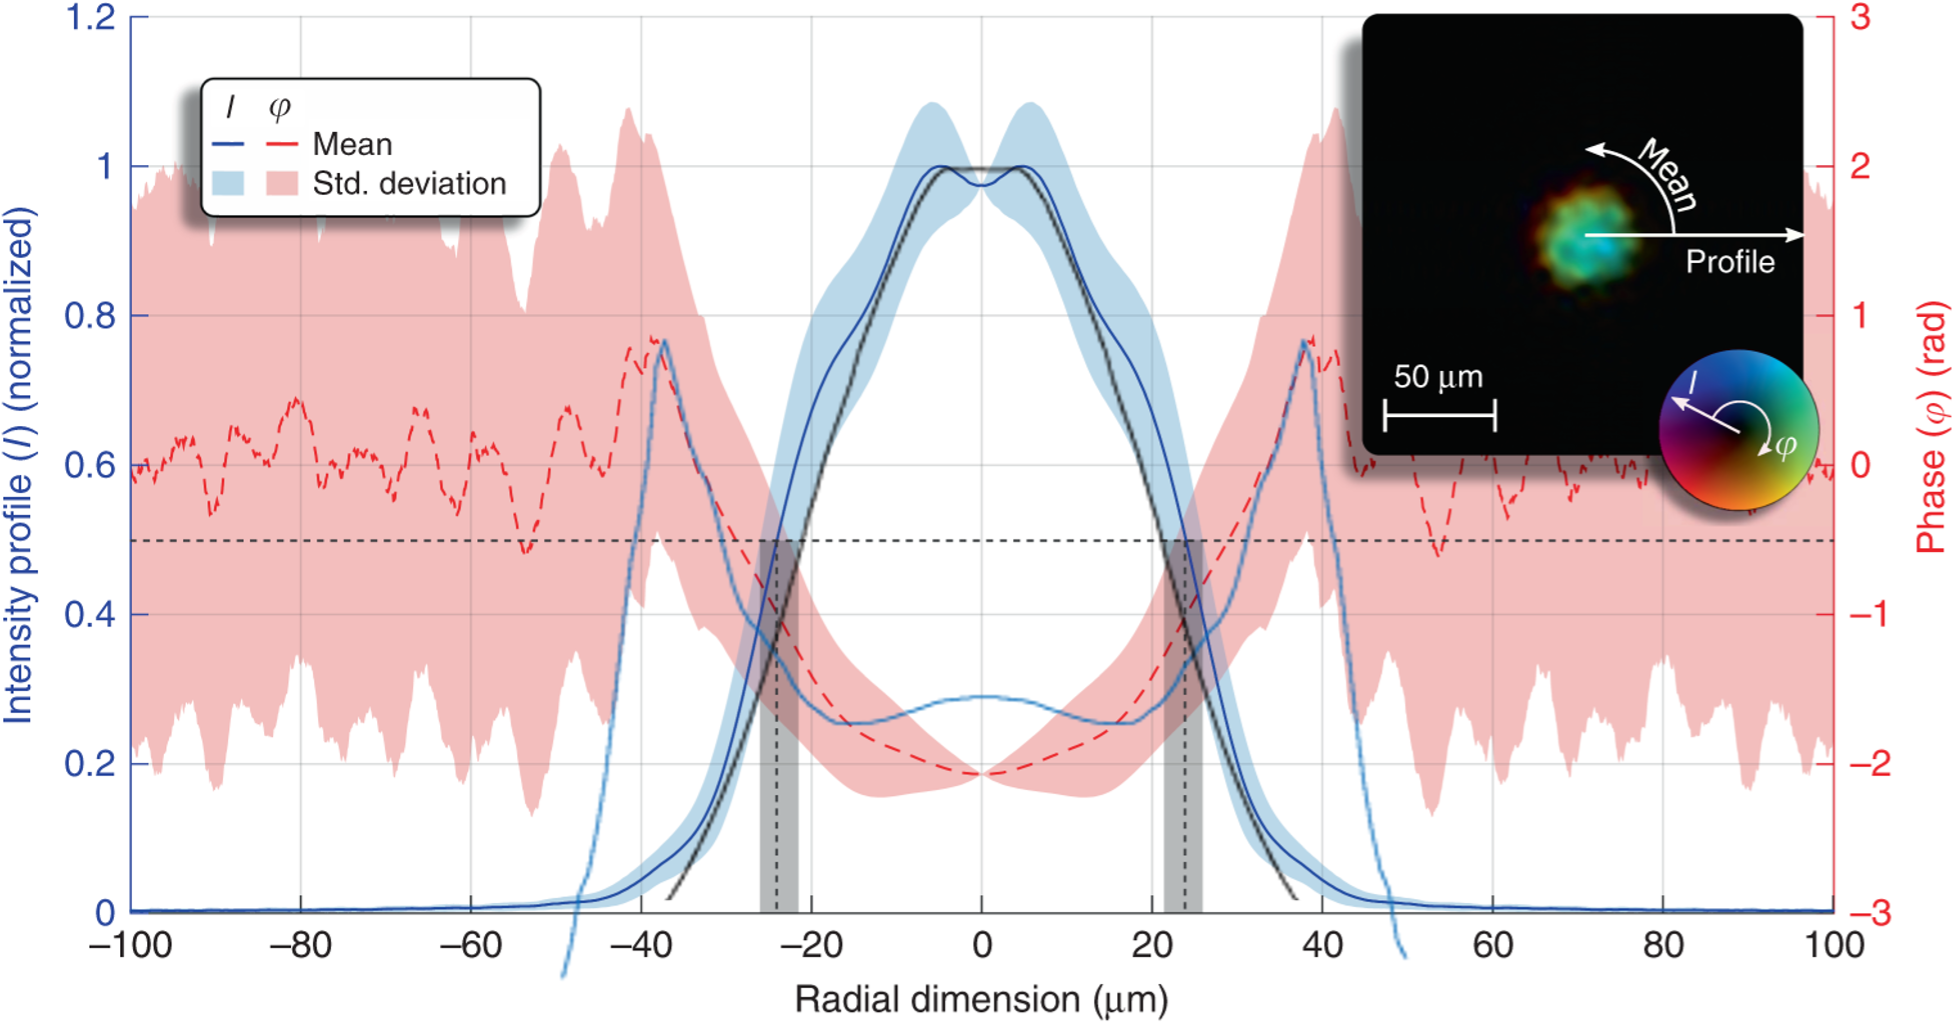
\includegraphics[width=0.75\textwidth]{Figuras/anx_cmp_40.png}
  \caption*{Comparación entre los perfiles radiales de intensidad--fase con $r_{i,min}=\qty{0}{µm}$, $r_{i,max}=\qty{5}{µm}$ y $\texttt{zshift}=0.75$; manteniendo los valores de los parámetros $k_{i}=\qty{50e6}{m^{-1}}$ y $z_{0i}=\qty{3.5}{mm}$; y el experimento.}
\end{figure}
